\documentclass[12pt, letterpaper, oneside]{ociamthesis}
\usepackage{algorithm}
\usepackage{algpseudocode}
\usepackage{amsfonts}
\usepackage{amsmath}
\usepackage[utf8]{inputenc}
\usepackage[english]{babel}
\usepackage{booktabs}
\usepackage[labelfont=bf]{caption}
\captionsetup[table]{position=top}
\usepackage{csquotes}
\usepackage{fancyhdr}
\usepackage{float}
\usepackage[margin=1.25in]{geometry}
\usepackage{graphicx}
\usepackage{url}
\usepackage{hyperref}
\usepackage[noabbrev, nameinlink]{cleveref}
\creflabelformat{equation}{#2\textup{#1}#3}
\usepackage{indentfirst}
\usepackage{listings}
\usepackage[numbers, comma, sort&compress]{natbib}
\usepackage{nomencl}
\usepackage{physics}
\usepackage{ragged2e}
\usepackage{setspace}
\usepackage{titlesec}
\usepackage{etoolbox}
\usepackage{wrapfig}
\usepackage{booktabs}
\usepackage{movie15}
\usepackage[nottoc,numbib]{tocbibind}
\usepackage{blindtext}
\usepackage{fancyhdr}
\usepackage{tikz}
\usepackage{multicol}
\usepackage{multirow,bigdelim}
\usepackage{silence}
\usepackage{array}


\pagestyle{plain}
 
\makeatletter
\patchcmd{\ttlh@hang}{\parindent\z@}{\parindent\z@\leavevmode}{}{}
\patchcmd{\ttlh@hang}{\noindent}{}{}{}
\makeatother

\newcommand\hr{\par\vspace{-.5\ht\strutbox}\noindent\hrulefill\par}


\WarningFilter{latex}{Text page}

\usetikzlibrary{matrix,chains,positioning,decorations.pathreplacing,arrows, shapes.geometric}

\setlength{\nomlabelwidth}{2cm}

\renewcommand{\nomname}{List of Abbreviations}

\newcommand*{\Scale}[2][4]{\scalebox{#1}{$#2$}}%
\renewcommand{\arraystretch}{1.2}


\newcolumntype{L}[1]{>{\raggedright\let\newline\\\arraybackslash\hspace{0pt}}m{#1}}

\hypersetup{
    pdftitle={Learning a Latent Space for EEGs with Computational Graphs},
    pdfauthor={Radhakrishnan Thiyagarajan},
    colorlinks=true,
    linkcolor=black,
    filecolor=black,      
    urlcolor=black,
    citecolor=black
}

\titleformat{\chapter}[display]
  {\Huge\bfseries}
  {}
  {0pt}
  {\thechapter \ {\huge $\boldsymbol{\vert}$} }

\titleformat{name=\chapter,numberless}[display]
  {\Huge\bfseries}
  {}
  {0pt}
  {}   
\titlespacing{\chapter}{0pt}{-70pt}{40pt}

\crefname{lstlisting}{listing}{listings}
\Crefname{lstlisting}{Listing}{Listings}

\title{Learning a Latent Space for EEGs with Computational Graphs}   

\author{Radhakrishnan Thiyagarajan}
\college{Albert Nerken Schoool of Engineering}

\renewcommand{\submittedtext}{A thesis submitted in partial fulfillment \\ of the requirements for the degree of}
\degree{Master of Engineering}
\degreedate{April 4, 2018}

\makenomenclature


\begin{document}
\baselineskip=18pt plus1pt

\setcounter{secnumdepth}{3}
\setcounter{tocdepth}{3}

\pagenumbering{gobble}

\maketitle


\addcontentsline{toc}{chapter}{Title Page}

\phantomsection
\begin{approval}
		
	\begin{centering}		
		\textsc{THE COOPER UNION}\\
		\textsc{ ALBERT NERKEN SCHOOL OF ENGINEERING }	
	\end{centering}
		
		
	\begin{flushleft}
		\justify
		This thesis was prepared under the direction of the Candidate's Thesis Adviser and has received approval. It was submitted to the Dean of the School of Engineering and the full Faculty, and was approved as partial fulfillment of the requirements for the degree of Master of Engineering.
	\end{flushleft}
		
	\bigskip
		
	\begin{flushright}
		\SignatureAndDate{Professor Richard Stock - Date}\\
		Dean, School of Engineering
				
	\end{flushright}
		
	\smallskip
		
	\begin{flushleft}
		\SignatureAndDate{Professor Sam Keene - Date}\\
		Candidate's Thesis Adviser
				
	\end{flushleft}
		
\end{approval}
\addcontentsline{toc}{chapter}{Signature Page}

\phantomsection
\begin{acknowledgements}
		
	Thanks to my advisor, Dr. Sam Keene, for the guidance, the encouragement and the friendship that he has provided me with throughout my time at The Cooper Union. 
		
	\smallskip
		
	Thanks to Chris Curro for teaching me deep learning, helping me improve my \LaTeX ing skills, and coauthoring my first paper. 
		
	\smallskip
		
	Thanks to my project partner, Zhengqi Xi, who worked with me last year and helped me get this project off the ground.
		
	\smallskip
		
	Thanks to the electrical engineering faculty at The Cooper Union for educating me in electrical engineering.
		
	\smallskip
	Thanks to Temple University for providing me their dataset for research. 
	
	\smallskip
	Thanks to my mentors, Shan and Nirmala, for helping and advising me in multiple ways during the past four years. 
		
	\smallskip
		
	Thanks to my friends, Abhinav, Ben, Tushar, Miles, Garo, Amy and Anish for standing by me and supporting my throughout these four years. 
		
	\smallskip
		
	Thanks to my parents, Thiyagarajan and Latha, and my younger brother, Abhiram, for encouraging me with their best wishes. 
		
			
\end{acknowledgements}

\addcontentsline{toc}{chapter}{Acknowledgements}

\begin{abstractlong}
	Despite the recent advances in data organization and structuring, electronic medical records (EMRs) can often contain unstructured raw data, temporally constrained measurements, multichannel signal data and image data. Cohort retrieval, the action of finding a group of observations with similar properties, of these signals will allow us to compare and contrast the signals in large quantities We present a proof of concept system that can alleviate this problem by mapping raw data to a compressed 64-dimensional space where the Euclidean distance between data is a measure of similarity. Using electroencephalographs (EEGs) as a case study, we optimize a deep neural network mapping from the spectrogram of EEG data to a latent space by using the triplet loss function. After this mapping, distance-based methods, such as nearest neighbors search, could be employed to find similar EEG records by treating the embeddings as the keys to the EEG signal in a database as part of a cohort retrieval system. To verify that this method learns a meaningful representation of the data, we apply a six-class k-NN classifier to the output, a binary (seizure-like and noise-like signal) k-NN classifier to the output and visualize the output latent space using the t-SNE dimensionality reduction technique. We achieve a $60.4\%$ six-class seizure classification accuracy, a $90.1\%$ binary seizure classification accuracy on the TUH EEG Cohorts dataset and observe distinct clusters in a reduced dimension latent space discovered using the t-SNE algorithm. 		
\end{abstractlong}

\begin{romanpages}
									
	\tableofcontents
	\listoffigures
	\listoftables
									
									
	\printnomenclature
	\addcontentsline{toc}{chapter}{List of Abbreviations \& Symbols}
									
									
\end{romanpages}

\pagenumbering{arabic}

\doublespacing

\pagestyle{fancy}
\fancyhead{}
\lhead{\leftmark}
\rhead{\thepage}

\chapter{Introduction}

The healthcare industry commonly stores diverse instrumentation signals such as EEGs\nomenclature{EEG}{Electroencephalography}, EKGs\nomenclature{EKG}{Electrocardiogram}, MEGs\nomenclature{MEG}{Magnetoencephalography}, X-Rays, MRIs\nomenclature{MRI}{Magnetic Resonance Imaging}, and CAT scans in a variety of digital formats commonly referred to as Electronic Medical Records (EMRs\nomenclature{EMR}{Electronic Medical Records}).  These records can also contain natural language notes from medical professionals. It is difficult to perform complex information retrieval on these records. Rich information retrieval may open up the ability to compare and contrast patient records en-masse leading to new understandings of disease pathologies. For example, while the healthcare industry possesses a large amount of data on Alzheimer's Disease, a common chronic neurodegenerative disorder, medical professionals are unable to find the underlying cause of this disease and why it worsens over time. If such data can be transformed into an accessible and patient invariant format such that different patients with similar cases can be found easily, medical professionals may be able to pinpoint the cause of the disease and discover better treatments. Towards this goal, \citet{piccone} have demonstrated a system that can automatically discover, time-align and annotate EEG events in order to perform cohort retrieval, the task of efficiently finding a group of observations that share defining characteristics given an example observation. The signal event detection and classification work in \citet{piccone} uses Hidden Markov Models, which have been shown to work well with sequential data. Although this model achieved $91.4\%$ sensitivity and $8.5\%$ specificity on the signal classification task, it is not possible to infer similarity of samples from the output of a classifier. Since similarity is a key factor in cohort retrieval, it is important to incorporate it into any cohort retrieval scheme.

In contrast to the work done by \citet{piccone}, we optimize a deep neural network using a triplet loss function that results in a reduced dimensionality latent space which minimizes the distance between similar signals and maximizes the distance between dissimilar signals. In doing so, we expect clusters of signals to form in the latent space characterized by features that have a meaningful interpretation of the original signals. At inference time, we can use the network to map new EEG signals onto this latent space for querying. New samples could be presented to this system and mapped into the latent space. After this mapping, clustering or other distance-based methods could be employed to find similar EEG records as part of a cohort retrieval system. It is hoped that this system can be used to discover significant relations between diseases in medicine.  

We organize the rest of this thesis in the following way. In \cref{bckgnd},  we discuss background information on machine learning needed to understand our work. In \cref{relwork}, we review the literature relevant to deep metric learning and deep feature embedding techniques. In \cref{dataresources}, we describe our data and how we organized it for ease of access. In \cref{expres}, we describe our final models, their quantitative and qualitative characteristics, our experimental results and our analysis of those results. 

\chapter{Background}
\label{bckgnd}

\section{ Machine Learning}
Machine learning is the field of computer science that allows computers to acquire knowledge from data and make some sort of prediction or estimation without explicitly programming said knowledge \cite{bishop_2013}. \citet{ai_text_book} say that a machine learning algorithm is designed for a particular task or problem, and is said to be learning if it improves its performance at that task based on a metric. Machine learning is often used for tasks that require pattern recognition, especially in large amounts of data.  Examples of such tasks include handwriting recognition, cybersecurity breach detection, medical disease diagnosis and autonomous cars control systems \cite{lecun1998mnist,cybersecurity,3d_conf_for_alzheimers,driverless_cars}. Due to the variety of tasks that could fit this broad definition, there are also a variety of approaches that could be used to solve each of those particular tasks.


\subsection{Supervised Learning}
\label{supervised}

Supervised learning is a task that tries to learn a model that maps from a domain of inputs to a range of outputs based on data on which the task has already been accomplished. Mathematically, if $\mathcal{S} =\{ ( \mathbf{X_i}, \mathbf{y_i} ) \ | \ i = 1...N\} \subset \mathcal{P}$, then the machine learning task may be to find a function ,$ \mathbf{\hat{y}} = f(\mathbf{X}) $, an estimate of $\mathbf{y}$ for any $(\mathbf{X}, \mathbf{y}) \in \mathcal{P}$ where $\mathbf{X}$ is an input, $\mathbf{y}$ is an output (also called a label or a target), $\mathbf{\hat{y}}$  is an estimate of the output from the machine learning model, $\mathcal{S}$ is a set of $N$ examples of input-output pairs called training set, and $\mathcal{P}$ is the population of input-output pairs. For example, in the case of the hand-written digits recognition using the data provided by \citet{lecun1998mnist}, the input $\mathbf{X}$ may be the image of the digit, $\mathbf{y}$ will be the true label of the digit provided by the dataset, and $\mathbf{\hat{y}}$ is the discrete value that the algorithm infers restricted to the range of $\mathbf{y}$. This particular process is called classification since we are restricted to a discrete set of values that are predefined. In order to learn a mapping from $\mathbf{X}$ to $\mathbf{y}$, a loss function, $J(\mathbf{y}, \mathbf{\hat{y}})$, can be used to quantify how well our model performs on our sample set, $\mathcal{S}$. In supervised learning, $J(\mathbf{y}, \mathbf{\hat{y}}) \rightarrow 0 \ \text{as} \ \mathbf{\hat{y}} \rightarrow \mathbf{y}$. If the loss function's value is large, the model is doing poorly; if the loss function's value is small, it generally means that the algorithm is doing well on $\mathcal{S}$. The loss function's value can be fed back to the algorithm to iteratively change the algorithm until the loss function's value reaches convergence or until it is stopped by the developer before complete convergence. Iteratively changing the model while keeping track of this loss function will allow for the model's input-output mapping to improve over time. 

\subsection{Unsupervised Learning}

The task of unsupervised learning is to discover some hidden patterns within the data without any prior knowledge or labels of any sort. 

One common task that is often seen in unsupervised learning is cluster analysis. Cluster analysis or clustering is the machine learning task of grouping a set of observations or objects in a way such that the portion of data in the same group (a cluster) is more similar than the portion that is not in the same group. Whereas classification tries to find a decision boundary between predefined classes, clustering tries to find decision boundaries in the sample space provided without knowing how many distinctive clusters there are in the dataset. Mathematically, if $\mathcal{S} =\{  \mathbf{X_i} \ | \ i = 1...N\} \subset \mathcal{P}$, then the machine learning task might be to find a function, $\mathbf{\hat{y}} = f(\mathbf{X})$, such that $\mathbf{\hat{y}} \in \{\mathbf{y_1}, \mathbf{y_2}, ...,\mathbf{y_k}\}$ where $k$ is the number of clusters that the algorithm finds. Notice how there is no dependency on a label as opposed to the classification task presented in \cref{supervised}. Clustering algorithms, such as the k-means algorithm developed by \citet{macqueen1967some}, may need a number, $k$, provided by a developer suggesting that there are $k$ clusters. However, the algorithm is not provided any knowledge on which cluster each data point in the dataset is from, which is why it is unsupervised. The clusters resulting from these types of algorithms are a matter of interest in many applications and can lead to natural ways of classifying things once the general trend is found in the input space.  

Another common task called dimensionality reduction attempts to use a set of observations with $M$ attributes and decreasing it to $K$ attributes where $M > K$, such that the characteristics of the original observation are still represented in the reduced vector space.  Mathematically, if $\mathcal{S} =\{ ( \mathbf{X_i} \in \mathbb{R}^{M\times1} ) \ | \ i = 1...N\} \subset \mathcal{P}$, then the machine learning task might be to find a function $\mathbf{\hat{y}} = f(\mathbf{X})$ where $\mathbf{\hat{y}} \in \mathbb{R}^{K \times 1}$ such that both $\mathbf{X}$ and $\mathbf{\hat{y}}$ accurately represent the original observation. A loss function, $J(\mathbf{X}, \mathbf{\hat{y}})$, may be defined to ensure that both $\mathbf{X}$ and $\mathbf{\hat{y}}$ represent the same observation. An example of dimensionality reduction is provided below. \Cref{fig:lennaoriginal} is a high-quality image of a kitten and you can clearly see that its a kitten in the image. We can down-sample this image to $64\times64$ pixels and can still see the kitten even though the image is distorted in \cref{fig:lennareduced}. Despite using $3 \times 2^{12}$ pixels for the compressed image as opposed to $3 \times 2^{18}$ pixels for the original image, we are still able to see what the image represents. Hence, down-sampling is a crude example of dimensionality reduction. 

\begin{figure}[!htbp]
	\centering
	\begin{minipage}[b]{0.45\textwidth}
		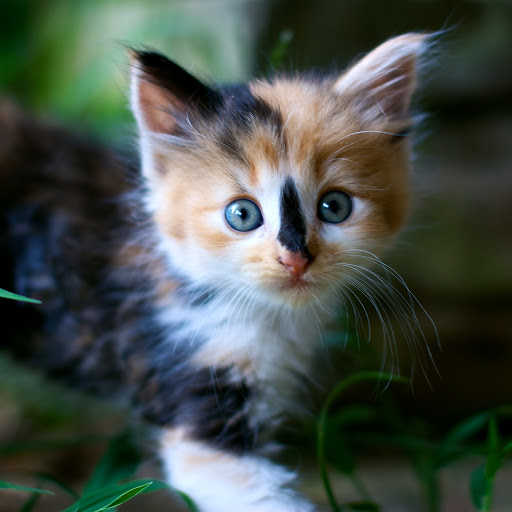
\includegraphics[width=\textwidth]{pictures/kitten.jpg}
		\caption[Original resolution photograph of a kitten]{Original $512\times512$ pixels photograph of a kitten \cite{travers_2009}}\label{fig:lennaoriginal}
	\end{minipage}
	\hfill
	\begin{minipage}[b]{0.45\textwidth}
		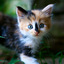
\includegraphics[width=\textwidth]{pictures/KittenDown.jpg}
		\caption[Reduced resolution photograph of a kitten]{Down-sampled $64\times64$ pixels photograph of a kitten}\label{fig:lennareduced}
	\end{minipage}
\end{figure}

Often, dimensionality reduction techniques are used to learn latent variables, which  are variables that are not directly observed. For example, in a picture of a kitten, a latent variable might be the cuteness of a kitten. Cuteness is not something that can be directly observed. A kitten can be observed to have a certain length of fur, a certain color of fur, eye diameter to head ratio, etc. but it is difficult to quantify a kitten's cuteness numerically. Whereas humans are able to claim a kitten is cute and can have a general consensus on it after looking at an image of a kitten, a machine might be able to learn what cuteness is by reducing the dimensionality of data and understanding it at a lower dimensional level but at a higher level of abstraction. These latent variables, along with other variables, can be used as input features to another machine learning algorithm which could be used learn more about the data. Hence, dimensionality reduction leads to processes known as feature extraction and feature engineering, the process of finding important variables derived directly or indirectly from raw input. Generally, the set of features that arise from feature extraction and engineering can form what is called a latent space (also called feature embedding, embedding space, latent space or space). The latent space is able to represent data that may have originally been incomparable by a machine as comparable points in this latent space. 

% \subsection{Feature Extraction \& Feature Engineering}

% Feature extraction is widely defined by \citet{bishop_2013} as the task of preprocessing the original input variables to transform them into some new domain space where it is hoped that pattern recognition and other machine learning problems are easier to solve. Any new data that is to be passed through the machine learning algorithm in the future would need to be transformed in the same way as the rest of the data. For example, the MNIST dataset, provided by \citet{lecun1998mnist}, is a database of handwritten numeric digits from the English language. If we are trying to identify these digits, a typical way to extract features from this image would be to translate, scale, rotate and normalize the images pixels so that the input into our algorithm is spatially invariant. In this case, each image is $28 \times \ 28$ pixels images of digits and every pixels' value in the image can be used as input into the value. This often leads to extra information that is not always needed or useful for the algorithm and can in fact hinder the algorithm's ability to find the best solution possible.

% %  lead to a phenomena defined as over fitting where the machine learning algorithm essentially memorizes the data that it was shown (known as the training data), does not generalize to data that it has not seen before (known as testing data) and might ultimately be more erroneous than we might hope for.
% Therefore, feature extraction itself does not suffice when looking at machine learning algorithms; it is as important to select and construct new features from the original data's features as much as it is to select the right algorithm.

% Feature engineering is therefore the process of using domain knowledge, the understanding of a particular dataset and what features are generally important in the data dataset, to select and create features that have the potential to simplify the data as seen by the machine learning model and therefore, simplify the complexity of the machine learning model that results. Once these features are decided on and extracted from the raw data, it can be fed into machine learning algorithms for predictive analysis. There are multiple ways that this can be done. Typically, experts that have domain knowledge of the data tend to look at the data, manually identify potentially useful features, and use computer programming to transform the dataset as a whole so that it reflects these features. For example, in the case that we are attempting to classify a set of images of tumors as malignant or not, an expert in radiology and tumors may be needed to find features such as color or intensity that are important in identifying the characteristics of a tumor that might indicate that the tumor is malignant or not. This process takes a lot of time, effort and frankly is less automated than it could be. However, with the advent of some more advanced algorithms, it becomes possible to automatically learn the features that are important. One of these advanced algorithms utilizes artificial neural networks and deep learning to learn these features.

\subsection{Parametric Modeling and Optimization}
\label{paramsmodeling}

Although the different types of learning methods have been described, we still need a way to train these models. One way to do this is to restrict our function $f$ representing the machine learning algorithm to a function that is parametric and differentiable. By changing the parameters of the function, we hope to make it better in the task that we designed it for. Therefore, we augment our original functional form of our machine learning model, $\mathbf{\hat{y}} = f(\mathbf{X})$, and refer to it as $\mathbf{\hat{y}} = f(\mathbf{X} \ | \ \boldsymbol{\theta})$  where $\boldsymbol{\theta}$ is a vector of parameters of the given function and $f$ is a differentiable function with respect to $\boldsymbol{\theta}$. Hence, our goal would be to find a $\boldsymbol{\hat{\theta}}$ that minimizes the loss function, $J(\mathbf{y}, f(\mathbf{X} \ | \ \boldsymbol{\theta}))$. The best way to approach this problem would be to calculate the gradient with respect to $\boldsymbol{\theta}$, set it equal to zero and solve for a $\boldsymbol{\hat{\theta}}$ like so

\begin{equation}
	\nabla_{\boldsymbol{\theta}} J(\mathbf{y}, f(\mathbf{X} \ | \ \boldsymbol{\theta})) = 0.
\end{equation}

However, in many cases, it is either not possible to find a closed form solution or the way to do so becomes intractable, especially when the training set is large. Often, the gradient calculation with respect to the model's parameters are estimated and are not exact. Hence, instead of attempting to find an analytic solution, we must use gradient descent, a numerical optimization algorithm, by finding the direction of steepest descent and moving the parameters in that direction in the following way 

\begin{equation}
	\label{eq:sgd}
	\boldsymbol{\theta}_{t+1} \leftarrow \boldsymbol{\theta}_t - \eta \ \nabla_{\boldsymbol{\theta}} J(\mathbf{y}, f(\mathbf{X} \ | \ \boldsymbol{\theta})) 
\end{equation}

\noindent
where $\eta$ is the learning rate hyperparameter that controls the size of the step towards the direction of steepest descent as described by \citet{gd_explanation}. If this parameter is too large, the step towards the optimal $\boldsymbol{\theta}$ will overshoot, miss the optimal $\boldsymbol{\theta}$ and never converge. If this parameter is too small, the step towards the optimal $\boldsymbol{\theta}$ will be more precise, but the time to find $\boldsymbol{\hat{\theta}}$ will be large. One way to solve this problem is to change the learning rate over time so that in the beginning large steps are taken and when the amount of change in between $\boldsymbol{\hat{\theta}}_{t}$ and $\boldsymbol{\hat{\theta}}_{t+1}$ is small, the learning rate is decreased as proposed by \citet{decreasing_learning_rate} in order to get as close to the optimum solution as possible. Gradient descent is the name that is usually given to the algorithm which calculates the gradient based on the entire training set and updates the parameters using that gradient value. Another form of gradient descent, stochastic gradient descent (SGD\nomenclature{SGD}{Stochastic Gradient Descent}) developed by \citet{sgd1} and \citet{sgd2}  calculates the gradient either for a single sample or a small batch of samples and takes small steps towards the optimal solution. SGD is computationally faster. Since large datasets cannot be held in RAM, it is faster to select mini-batches of data from the training set and calculate the gradient on said mini-batches. SGD is able to make more updates over a time period than gradient descent and results in a model as good as or better than that of gradient descent. Generally, this process is repeated multiple times on the training data and each repetition is called an \textit{epoch}.

Unfortunately, as the number of parameters that the equation needs to train increases, the classic SGD algorithm becomes insufficient. The algorithm finds parameters which are local minimums in the function $J$ as opposed to global minimums. An example of a global minimum and local minimum is shown in \cref{fig:minmax}. Consequently, the model that results is not as optimal as it can be. More sophisticated algorithms have been developed over time. One of these algorithms is called Adam and was developed by \citet{kingma2014adam}. 

\begin{figure}[!ht]
	\centering
	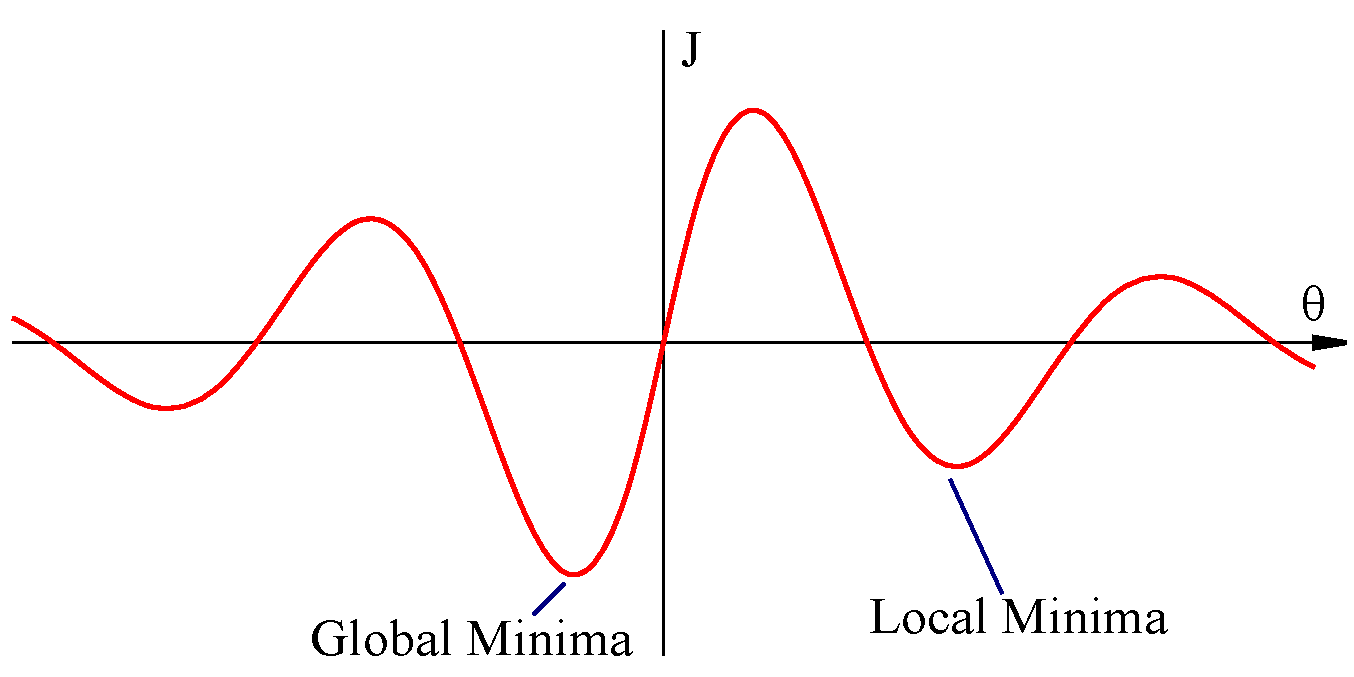
\includegraphics[width=0.45\linewidth]{pictures/minmax.pdf}
	\caption{Illustration of global minimum vs. local minimum}\label{fig:minmax}  
\end{figure}

Adam, the short form for Adaptive Moment Estimation, is a first-order optimization algorithm that uses running averages of the gradient as well as the  bias-corrected estimates to update the first two moments of the gradient to update the parameters $\boldsymbol{\theta}$. Moments are the measures of how the gradient has changed over the last couple of iterations,  The moment allows the optimization algorithm to act like a ball on a hill trying to roll to the lowest height possible. The ball will continue to roll even if a local minimum is achieved and continue to try to find a global minimum. In the case that the minimum that it finds \textit{is} the global minimum, the ball will continue to oscillate around that point until it loses momentum. Adam works in an analogous way. Therefore, we use Adam in our experiments as opposed to classic SGD for optimizing our models. 

\subsection{Bias-Variance Trade-off}
\label{bias_variance_tradeoff}

One of the main goals of machine learning is to learn a general trend from a limited amount of sample data. In other words, we expect training accuracy, i.e. the predictive accuracy of the model on the training set, and the testing accuracy, i.e. the predictive accuracy of the model on unseen data from the real world, to be as close as possible. Unfortunately, this is not always the case. \Cref{fig:overfit} demonstrates this concept by fitting a first and a twentieth-degree polynomial to the same data originating from a sinusoid using the least squares loss function given by \cref{eq:leastsquares}. 

\begin{equation}
	\label{eq:leastsquares}
	J(\mathbf{y}, f(\mathbf{X} \ | \ \boldsymbol{\theta})) = \sum_{i=0}^{N} (\mathbf{y}_i  - f(\mathbf{X} \ | \ \boldsymbol{\theta}_i))^2
\end{equation}


It is evident from \cref{fig:overfit} that the twentieth-degree polynomial tries to go through as many points as possible and ends up over-fitting the data. On the other hand, the first-degree polynomial tries to best fit the data but is unable to do so due to the lack of complexity and, therefore, under-fits the original data. Neither of these graphs represents the true nature of the sinusoid. Therefore, we are faced with a trade-off between two sources of errors: bias and variance. 

\begin{figure}[!ht]
	\centering
	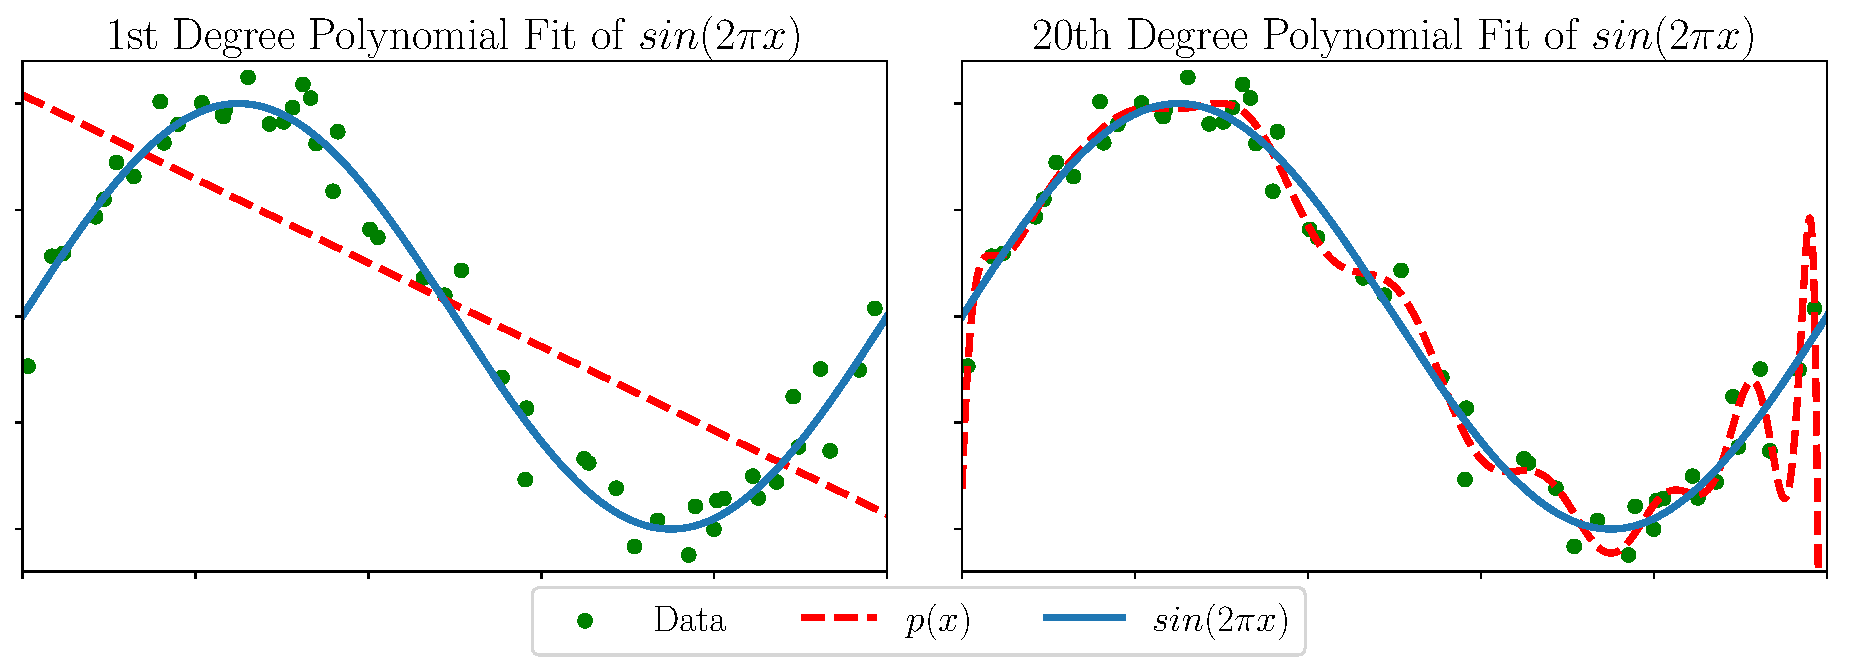
\includegraphics[height=0.35\linewidth]{pictures/poly_fit.pdf}
	\caption[Example of an under-fit and an over-fit model]{Example of an under-fit (left) and an over-fit (right) model}\label{fig:overfit}  
\end{figure}

Bias is the error that arises from making overly simplistic assumptions about the underlying trend in the data and results from using too few parameters in the model we are training. Variance is the error that arises from making overly complicated assumptions about the underlying trend in the data and results from using too many parameters in the model we are training. These two errors comprise the bias-variance trade-off. In order to minimize this error, we need to make a compromise between these two sources of error and select a model that is neither too complex nor too simple.

\begin{figure}[!ht]
	\centering
	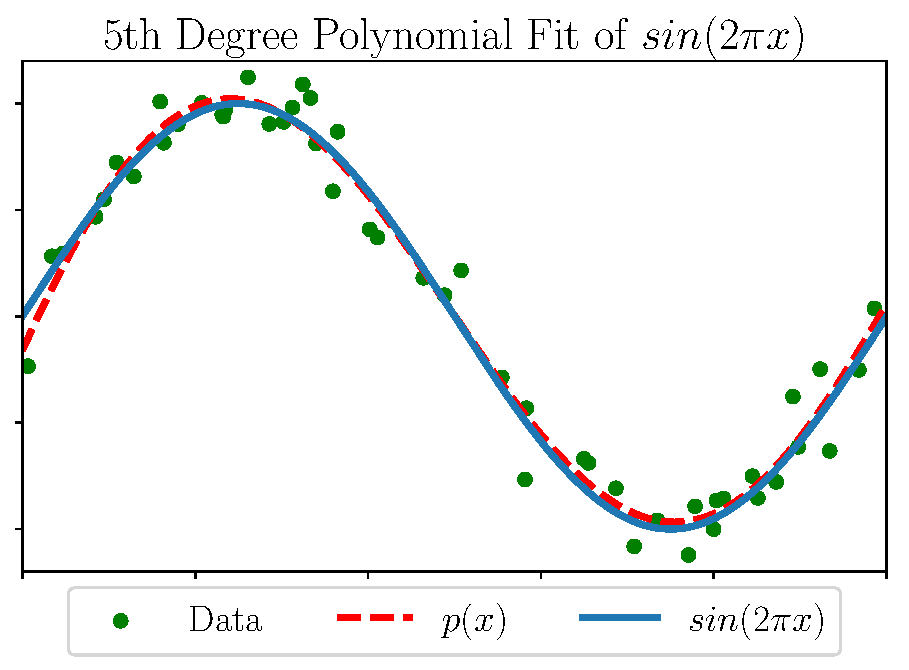
\includegraphics[height=0.35\linewidth]{pictures/poly_fit_correct.pdf}
	\caption{Example of a well-fit model}\label{fig:wellfit}  
\end{figure}

There are two ways that we can approach this problem. Either we can start with a simplistic model and make it more complex or we can start with a complex model and make it simpler. The latter is easier and the general name given to the process of making a relatively complex model simpler is called regularization. An example of a well-fit polynomial fit after simplifying the twentieth-degree polynomial is shown in \cref{fig:wellfit}.

In order for regularization to work, we need to know whether the model is generalizing well or not. Hence, we split the original training set, $\mathcal{S}$ into two mutually exclusive sets $\mathcal{S}_t$, the training set the model uses to learn, and $\mathcal{S}_v$, the validation set which we can use to see if the model is generalizing well to data that it has not seen before. If the validation accuracy is significantly lower than the training accuracy, we can infer that the model is not generalizing well.

One way we can regularize the model is by adding a penalty term to the loss function, $J(\mathbf{y}, f(\mathbf{X} \ | \ \boldsymbol{\theta}))$, based on the values of $\boldsymbol{\hat{\theta}}$. The resulting loss function would then be

\begin{equation}
	J_{t}(\mathbf{y}, f(\mathbf{X} \ | \ \boldsymbol{\theta})) = J(\mathbf{y}, f(\mathbf{X} \ | \ \boldsymbol{\theta})) + \lambda \ P(\boldsymbol{\theta})
\end{equation}

\noindent
where $\lambda$ is a hyperparameter that controls how much we want to penalize a complex model and $P$ is a function such that $P(\boldsymbol{\theta}) \rightarrow \infty \text{ as } \theta_i \rightarrow \infty$. The two equations shown below are examples of such penalties. 


\begin{equation}
	\label{eq:l1}
	P(\boldsymbol{\boldsymbol{\theta}}) = \sum_{k = 1}^{N}{|\theta_k|}
\end{equation}

\begin{equation}
	\label{eq:l2}
	P(\boldsymbol{\theta}) = \sum_{k = 1}^{N}{\theta_k^2}
\end{equation}


\Cref{eq:l1} is known as the $L_1$ penalty and promotes sparsity. This means that the penalty forces any parameter that does not contribute to the model to zero thereby reducing the total number of parameters involved in the model. $L_2$ penalty, shown in \cref{eq:l2}, on the other hand, minimizes the contribution of a parameter but it does not force it to zero. Therefore, the number of parameters tends to be high, but the overall complex nature of the model is reduced. It is important to tune the hyperparameter $\lambda$ based on validation results in order to accurately penalize complex models to find a trade-off between bias and variance. 

%%TODO: Add cross-validation blurb here

\section{Neural Networks \& Deep Learning}

Artificial Neural Networks (ANNs\nomenclature{ANN}{Artificial Neural Network}), also called neural networks, are a type of computational system that was originally inspired by biological neural networks found in organisms that have a nervous system. Neural networks are at the cutting edge of difficult machine learning tasks and have surpassed human-level performance in these tasks. Neural networks have been used to solve a variety of problems including those in computer vision, speech recognition, machine translation, video game bots and medical diagnostics \cite{imagenet_cnn,acoustic_modeling_speech,neural_translation,atari_deep_reinforcement_learning,3d_conf_for_alzheimers}.

\subsection{Motivation for Neural Networks}

Neural networks were originally inspired by biological neurons. Biological neurons generally consist of a cell body, dendrites, synapses and an axon. A dendrite is a part of a neuron that receives signals from other cells, including neurons, which were transmitted through a synapse as a chemical signal. These received signals are then propagated towards the cell body as an electrical signal. Once the cell body receives this electrical signal, more reactions happen within the cell body. If a certain action potential is reached, the neuron that received the signal fires and propagates the received signal along its axon towards other neurons and cells. A figure of a biological neuron is shown below in \cref{fig:bioneuron}. The biological nervous system is, in essence, a network of these cells interconnected with each other in various ways. 

\begin{figure}[!ht]
	\centering
	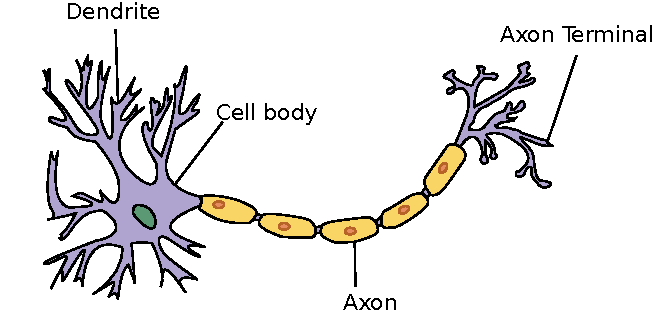
\includegraphics[height=0.35\linewidth]{pictures/Neuron.pdf}
	\caption[Illustration of a biological neuron]{Illustration of a biological neuron\cite{wiki:neuronpic}}\label{fig:bioneuron}  
\end{figure}

An artificial neural network tries to mimic a nervous system through the simulation of neurons. A visual representation of a single artificial neuron or node is shown in \cref{fig:activationblockdiagram}.  The inputs, $\{x_1 ... x_n\}$, are the set of numbers either given directly to the neuron or resulting from other neurons in the network. The neuron then multiplies each of these inputs by a corresponding weight $\{w_1 ... w_n\}$ and then sums these values together and adds a bias value $b$. The neuron then applies an activation function, $\sigma$, and delivers its result through its axon to the next neuron or neurons in the network. Types of activation functions are discussed in \cref{activationfunctions}. 

\begin{figure}[!ht]
	\centering
	\begin{tikzpicture}[
			init/.style={
				draw,
				circle,
				inner sep=2pt,
				font=\Huge,
				join = by -latex
			},
			squa/.style={
				regular polygon,
				regular polygon sides=4,
				draw,
				inner sep=0.3em,
				font=\Large,
				join = by -latex
			},
			start chain=2,node distance=13mm
		]
		\node[on chain=2] 
		(x2) {$x_2$};
		\node[on chain=2,join=by o-latex] (w2)
		{$w_2$};
		\node[on chain=2,init] (sigma) 
		{$\displaystyle + $};
		\node[on chain=2,squa,label=above:{\parbox{2cm}{}}]   
		{$\sigma$};
		\node[on chain=2,label=above:{},join=by -latex] 
		{$y$};
		\begin{scope}[start chain=1]
			\node[on chain=1] at (0,1.5cm) 
			(x1) {$x_1$};
			\node[on chain=1,join=by o-latex] 
			(w1) {$w_1$};
		\end{scope}
		\begin{scope}[start chain=3]
			\node[on chain=3] at (0,-1.5cm) 
			(xn) {$x_n$};
			\node[on chain=3,label=below:{},join=by o-latex] 
			(wn) {$w_n$};
		\end{scope}
		\node[label=above:\parbox{2cm}{\centering $b$}] at (sigma|-w1) (b) {};
																		
		\draw[-latex] (w1) -- (sigma);
		\path (x2) -- (xn) node [black, font=\large, midway, sloped] {$\dots$};
		\path (w2) -- (wn) node [black, font=\large, midway, sloped] {$\dots$};
		\draw[-latex] (wn) -- (sigma);
		\draw[o-latex] (b) -- (sigma);
																		
		(x1.north west) -- node[left=10pt] {Inputs} (xn.south west);
	\end{tikzpicture}
	\caption{Block diagram of a single artificial neuron}\label{fig:activationblockdiagram}  
\end{figure}

As described in \cref{paramsmodeling}, training a model is optimizing its learnable parameters, $\boldsymbol{\theta}$. The same concept applies to neural networks. The primary learnable parameters of the neural network are its weights. Depending on the architecture, i.e. the what parts the neural network is made up of, it may be possible to learn parameters presented in other parts of the neural network, such as the activation function. The process of learning any of these parameters for a neural network is called backpropagation. 

Backpropagation begins with the forward propagation of a set of inputs. Forward propagation is when a neural network infers the output for a particular set of inputs. The network propagates the inputs, $\mathbf{X}$, through each appropriate neuron in a neural network sequentially depending on the architecture until the propagation reaches the output neuron, which will result in $\mathbf{\hat{y}}$. The output neurons' results can be compared to the true output $\mathbf{y}$ and, unless the network is already trained, a significant amount of error is expected between $\mathbf{y}$ and $\mathbf{\hat{y}}$, which can be quantified by a loss function, $J(\mathbf{\hat{y}}, \mathbf{y})$. A large loss indicates that the parameters need to be optimized which means that each of the unoptimized parameters contributes a small error to the total error in the output. Therefore, we need to trace back the steps in the neural network and find the amount of error that each weight contributes for each input sample and adjust the respective weights. In other words, we are propagating the error backward towards every learnable parameter in the network, which is essentially the gradient of the loss function. Hence, \cref{eq:sgd} can be used to train the network. 

% \subsection{Types of Neural Networks}

\subsection{Fully Connected Feed-Forward Networks}

A fully connected neural network (FC network\nomenclature{FC}{Fully Connected Neural Network}) is a neural network that propagates a signal layer by layer. The first layer in a neural network is commonly called the input layer since all the activations are inputs given to the network by the user. Depending on what the neural network is being used for, any of the next layers can be considered an output layer. In general, the last layer is considered the output layer. Any node not in either the input layer or the output layer are considered hidden nodes since these nodes' values do not matter to the input or the output; they are simply nodes that transfer information to the next layer or the next node. The neural network is considered to be a feed-forward network because the network does not propagate the information backward to previous nodes for any feedback. \Cref{fig:mlpillustrated} shows an illustration of a four-layer, fully connected, feed-forward neural network. The input layer contains four input nodes, both hidden layers contain five hidden nodes and the output layer contains three output nodes. The number of hidden layers and the number of nodes in each hidden layer are considered to be hyperparameters, parameters that can be controlled by the developer.

\def\layersep{2.5cm}
\def\finallayersep{7.5cm}
\def\hblayersep{5.0cm}
\begin{figure}[!ht]
	\centering
	\begin{tikzpicture}[shorten >=1pt,->,draw=black!50, node distance=\layersep]
		\tikzstyle{every pin edge}=[<-,shorten <=1pt]
		\tikzstyle{neuron}=[circle,draw=black!50,fill=none,minimum size=20pt,inner sep=5pt]
		\tikzstyle{input neuron}=[neuron];
		\tikzstyle{output neuron}=[neuron];
		\tikzstyle{hidden neuron}=[neuron];
		\tikzstyle{annot} = [text width=4em, text centered]
																		
		% Draw the input layer nodes
		\foreach \name / \y in {1/1,2/2.2,3/3.4,4/4.6}
		% This is the same as writing \foreach \name / \y in {1/1,2/2,3/3,4/4}
		\node[input neuron] (I-\name) at (0,-\y) {$ x_\name $};
																		
		% Draw the hidden layer nodes
		\foreach \name / \y in {1/1,2/2.2,3/3.4,4/4.6,5/5.8}
		\path[yshift=0.5cm]
		node[hidden neuron] (H-\name) at (\layersep,-\y cm) {};
																		
																		
		\foreach \name / \y in {1/1,2/2.2,3/3.4,4/4.6,5/5.8}
		\path[yshift=0.5cm]
		node[hidden neuron] (H2-\name) at (\hblayersep,-\y cm) {};
																		
		% Draw the output layer node
																		    
		\foreach \name / \y in {1/1,2/2.2,3/3.4}
		\path[yshift=-0.75cm]
		node[output neuron](O-\name) at (\finallayersep, -\y cm) {$y_\name$};
																		
		% Connect every node in the input layer with every node in the
		% hidden layer.
		\foreach \source in {1,2,3,4}
		\foreach \dest in {1,2,3,4,5}
		\path (I-\source) edge (H-\dest);
																		            
		\foreach \source in {1,2,3,4,5}
		\foreach \dest in {1,2,3,4,5}
		\path (H-\source) edge (H2-\dest);
																		
		% Connect every node in the hidden layer with the output layer
																		    
		\foreach \source in {1,2,3,4,5}
		\foreach \dest in {1,2,3}
		\path (H2-\source) edge (O-\dest);
																		
		% Annotate the layers
		\node[annot,above of=H-1, node distance=1.5cm] (hl) {Hidden layer 1};
		\node[annot,above of=H2-1, node distance=1.5cm] (hb) {Hidden layer 2};
		\node[annot,left of=hl] {Input layer};
		\node[annot,right of=hb] {Output layer};
	\end{tikzpicture}
									
	\caption{Graph diagram of a four-layer neural network}\label{fig:mlpillustrated}  
\end{figure}

Fully connected feed-forward networks can be easily represented in mathematics as a series of matrix multiplications and activation functions. If there are $K$ layers in this type of neural network, there will be $K-1$ weight matrices and $K-1$ bias vectors. Each weight matrix will have an entry for a weight from a neuron in the previous layer to a neuron in the current layer. In other words, if there are $N$ neurons in the previous layer and $M$ neurons in the current layer, there will be $N \times M$ entries in the weight matrix and $1 \times M$ entries in the bias vector. For example, the output of the neural network shown in \cref{fig:mlpillustrated} will be 

\begin{equation}
	\mathbf{\hat{y}} = \sigma(\sigma(\sigma(\mathbf{x} \times \mathbf{W_1} + \mathbf{b_1}) \times \mathbf{W_2} + \mathbf{b_2}) \times \mathbf{W_3} + \mathbf{b_3})
\end{equation}

\noindent
where $\sigma$ is the activation function that acts on a matrix entry by entry, $ \mathbf{x} \in \mathbb{R}^{1 \times 4} $ for an input with one sample, $\mathbf{W_1} \in \mathbb{R}^{4 \times 5}$, $\mathbf{b_1} \in \mathbb{R}^{1 \times 5}$, $\mathbf{W_2} \in \mathbb{R}^{5 \times 5}$, $\mathbf{b_2} \in \mathbb{R}^{1 \times 5}$,  $\mathbf{W_3} \in \mathbb{R}^{5 \times 3}$, and $\mathbf{b_3} \in \mathbb{R}^{1 \times 3}$. 

Backpropagation can be easily calculated for a simple FC network as demonstrated by \citet{ai_text_book}. 


\subsection{Convolutional Neural Networks}
\label{cnns}

Convolutional neural networks (CNNs\nomenclature{CNN}{Convolutional Neural Network}) are a class of networks that have been successful in the field of image processing. 

CNNs were also inspired by the biology of creatures that have vision. In $1965$, \citet{receptive_field} showed that cats contain neurons that respond to small regions of the field of vision. Assuming that the eyes are not moving, the concept of a receptive field, the particular region of vision that causes a single neuron to fire, was introduced. The concept of a receptive field is what led to what we know as a CNN.

CNNs attempt to learn shift-invariant characteristics in an input based on kernels, also called filters, which slide through the image and results in a filtered version of the original input image. The convolution computes the inner product of the kernel and the corresponding receptive field, saves the result to a new matrix known as the feature map, strides a particular length, and repeats the process until the entire input is convolved with the filter. \Cref{fig:convolution} shows an example of this process. The $3 \times 3$ kernel shown can be visualized as sliding over the input image represented as a $5\times5$ matrix. Note that a zero padding has been applied to the matrix so that the resulting feature map is the same size as the original image. However, it is also possible to forgo the padding and have the convolution result in a smaller sized feature map depending on the architecture of the neural network. The feature map is the result of the convolution and helps the network understand abstract patterns in the input, such as edges in the case of an image.   

\begin{figure}[!ht]
	\centering
	\begin{tikzpicture}
		\matrix (mtr)[matrix of nodes,nodes={inner sep=0pt,text width=0.8cm,align=center,minimum height=0.8cm, draw}]
		{
			0 & 0   & 0   & 0   & 0   & 0  & 0 \\
			0 & 0   & 21  & 0   & 0   & 0  & 0 \\
			0 & 85  & 71  & 0   & 0   & 0  & 0 \\
			0 & 250 & 231 & 127 & 63  & 3  & 0 \\
			0 & 250 & 252 & 250 & 209 & 56 & 0 \\
			0 & 250 & 252 & 250 & 250 & 83 & 0 \\
			0 & 0   & 0   & 0   & 0   & 0  & 0 \\
		};
																		    
		\node [below= 0.1cm of mtr-7-4.south] (lm) {$\bf Image$};
		\node [right= 3.5cm of lm] (km) {$\bf Kernel$};
		\node [right= 1.95cm of km] (km) {$\bf Feature \ Map$};
																		    
		\draw[very thick, red] (mtr-1-1.north west) rectangle (mtr-3-3.south east);
																		    
		\draw [ultra thick, fill=yellow, opacity=0.2] (mtr-2-2.north west) rectangle (mtr-6-6.south east);
																		
		\draw[line width=0.5mm, blue] (mtr-1-2.north west) rectangle (mtr-3-4.south east);
																		
		\node[right = 0.2em of mtr] (str) {$\ast$};
																		
		\matrix (K) [right=0.2em of str, matrix of nodes, nodes={inner sep=0pt,text width=0.8cm,align=center,minimum height=0.8cm, draw}]
		{
			0 & 0 & 1 \\
			0 & 1 & 0 \\
			1 & 0 & 0 \\
		};
																		
																		
		\node [right = 0.2em of K] (eq) {$=$};
		\matrix (ret) [right=0.2em of eq, matrix of nodes,nodes={inner sep=0pt,text width=0.8cm,align=center,minimum height=0.8cm, draw}]
		{
			0 & 106 & 71 & 0 & 0 \\
			106 & 321 & 231 & 127 & 63 \\
			321 & 481 & 379 & 313 & 212 \\
			481 & 629 & 565 & 462 & 306 \\
			502 & 502 & 459 & 306 & 83 \\
		};
																		
		\draw[very thick, red] (ret-1-1.north west) rectangle (ret-1-1.south east);
																		
		\draw[ultra thick, blue] (ret-1-2.north west) rectangle (ret-1-2.south east);
																		    
		\node[anchor=south east, inner sep=0.01em, purple] at (mtr-1-2.south east) (xx) {\scalebox{.7}{\hspace{-1.5em}$\times 0$}};
		\node[anchor=south east, inner sep=0.01em, purple] at (mtr-1-3.south east) (xx) {\scalebox{.7}{\hspace{-1.5em}$\times 0$}};
		\node[anchor=south east, inner sep=0.01em, purple] at (mtr-1-4.south east) (xx) {\scalebox{.7}{\hspace{-1.5em}$\times 1$}};
		\node[anchor=south east, inner sep=0.01em, purple] at (mtr-2-2.south east) (xx) {\scalebox{.7}{\hspace{-1.5em}$\times 0$}};
		\node[anchor=south east, inner sep=0.01em, purple] at (mtr-2-3.south east) (xx) {\scalebox{.7}{\hspace{-1.5em}$\times 1$}};
		\node[anchor=south east, inner sep=0.01em, purple] at (mtr-2-4.south east) (xx) {\scalebox{.7}{\hspace{-1.5em}$\times 0$}};
		\node[anchor=south east, inner sep=0.01em, purple] at (mtr-3-2.south east) (xx) {\scalebox{.7}{\hspace{-1.5em}$\times 1$}};
		\node[anchor=south east, inner sep=0.01em, purple] at (mtr-3-3.south east) (xx) {\scalebox{.7}{\hspace{-1.5em}$\times 0$}};
		\node[anchor=south east, inner sep=0.01em, purple] at (mtr-3-4.south east) (xx) {\scalebox{.7}{\hspace{-1.5em}$\times 0$}};
																		
	\end{tikzpicture}
	\caption{Illustration of a spatial convolution used in CNNs}\label{fig:convolution}  
\end{figure}
There are a few advantages in using CNNs over more traditional methods of image processing or FC networks. Suppose we are trying to classify the digits found in the MNIST dataset. Traditionally, a human is involved, hand-engineers filters that seem to work, and uses post-processing algorithms, which looks at the filtered image to finally classify it as a digit between zero to nine. However, the usage of neural networks, especially CNNs, has eliminated the need for hand engineering filters. Backpropagation has the ability to learn the weights just like it has the ability to learn the weights of a FC network. However, learning the weights of CNNs still take a long time due to the current hardware capabilities. The inference time of CNNs is also generally longer thant hat of traditional algorithms. Hence, if time is not of the essence, CNNs tend to be better than classical algorithms for image processing tasks.

It is also better to use CNNs over FC networks for a task where spatially invariant features may be involved. Assume again that we are trying to classify the digits found in the MNIST dataset. In a single digit, there are $28 \times 28$ pixels with values between $0$ to $255$. For a fully connected network, all of these pixels would be input nodes and therefore there would be $28 \times 28 = 784$ input neurons. Assuming that the first hidden layer has $250$ neurons, the weight matrix will have $784 \times 250 = 196000$ weights that will have to be trained. This is an enormous amount of weights for a relatively small input size. However, if we use a convolutional layer with a $5 \times 5$ kernel on the same MNIST dataset, we would only have to train $25$ weights which means that the overall complexity of our network will go down and since we are learning a general trend, the average accuracy will go up. 

Series of convolutions can be placed sequentially after one another and gives the network a chance of learning more complicated spatial features that affect the final output. Networks that use series of convolutions one after another are commonly called deep convolutional neural networks or DCNNs\nomenclature{DCNN}{Deep Convolutional Neural Networks}. This is where the idea of deep learning arises since we are trying to increase the depth, the number of layers in a neural network, to learn more meaningful representations of data. 

%\subsection{Other Neural Network Operations}

\subsection{Pooling}
Pooling is a non-linear, sub-sampling operation in DCNNs which are used to reduce dimensions and the number of inputs to the subsequent layer. Pooling operations are non-parametric and they usually operate on the feature maps provided by convolutional layers before it. Two common types of pooling operations are used in neural networks: max-pooling and average pooling. Max-pooling \cite{scherer2010evaluation} finds the maximum element in a receptive field while average pooling takes the average of elements in the receptive field. Pooling is used in situations where the absolute location of features do not matter as much as the relative location of features.

\subsection{Dropout}
Dropout is a special type of regularization used in neural networks. The technique was motivated by the fact that both biological and artificial neurons make decisions based on the decisions of its predecessors. In the case that one of the predecessors of a particular neuron fires incorrectly, the current neuron is also more likely to fire incorrectly. In order to prevent this phenomenon, \citet{dropout} proposed this method of regularization which randomly zeros out a neuron's output based on a Bernoulli trial probability of $p$ for the current iteration of training. As a result, when a future neuron fires, its dependency on the previous neurons effectively decreases and has a better chance of learning a meaningful representation of the dataset. 


\subsection{Activation Functions}
\label{activationfunctions}

Several common activation functions are used today in cutting edge deep learning work. Our paper uses two of these activation functions: sigmoids and ReLUs. 
\subsubsection*{Sigmoid Activation}

The sigmoid activation has a functional form as follows: 

\begin{equation}
	\sigma(x) = \frac{1}{1 + exp(-x)}
\end{equation}

\noindent
and the corresponding gradient is 

\begin{equation}
	\sigma ' (x)  = \frac{exp(x)}{(exp(x) + 1)^2}.
\end{equation}. 

Brief analysis of the sigmoid's gradient shows that it suffers from the vanishing gradient problem, which refers to the function's gradient approaching zero as the input, $x$, increases or decreases. Because of this, sigmoid activations lead to extremely small gradient valules and tend to slow down learning. However, sigmoids are very useful for final layers, especially in classification problems, since they limit output values to less than one. They are also commonly used in probability since the cumulative distribution function (CDF) of various probability distributions are sigmoidal in nature. As a result, the multi-dimensional analog of the sigmoid function, the softmax function, is used in neural network classification tasks to predict the probability that a given input is a particular class. 

\subsubsection*{ReLU}

Rectified Linear Units (ReLU\nomenclature{ReLU}{Rectified Linear Units}) have demonstrated performance increases in both accuracy, generalization and training speed in neural networks as shown by \citet{dahl2013improving}. ReLU has a functional form of:

\begin{equation}
	\rho(x) = max(x, 0)
\end{equation}

\noindent
and the corresponding gradient is 

\begin{equation}
	\rho'(x) =  \begin{cases} 
		
	0 & x \leq 0 \\
	1 & x > 0 \\
	\end{cases}.
\end{equation}

\noindent It is noticeable that the functional form of ReLU's gradient is a step function and only takes values of either 1 or 0. As a result, networks with ReLUs do not have to deal with vanishing gradient or the exploding gradient problems and leads to a faster learning network.


% \subsubsection*{Leaky ReLU \& PReLU}

\section{Basics About EEG Signals}

The brain and the nervous system function on the basis of electrochemical reactions through biological neurons, as illustrated \cref{fig:bioneuron}, to send various signals to cells all over the body. Electroencephalography or EEG is a non-invasive way of measuring that electrical activity resulting on the surface of the brain due to these neurons. These signals can be used to diagnose seizures, brain tumors, head injuries, strokes, anesthesia overdose and many more ailments originating from the brain as described by \citet{mayo_eegs}.

According to \citet{eegs_info}, electrodes that measure voltage with respect to ground are attached to certain locations on the scalp as described by the $10$-$20$ system. An illustration of the $10$-$20$ system's placement map is shown in \cref{fig:tentwenty}. The letters and numbers on each of these electrodes can be used as an indication of location for each of the twenty-one channels in the EEG. 

\begin{figure}[!ht]
	\centering
	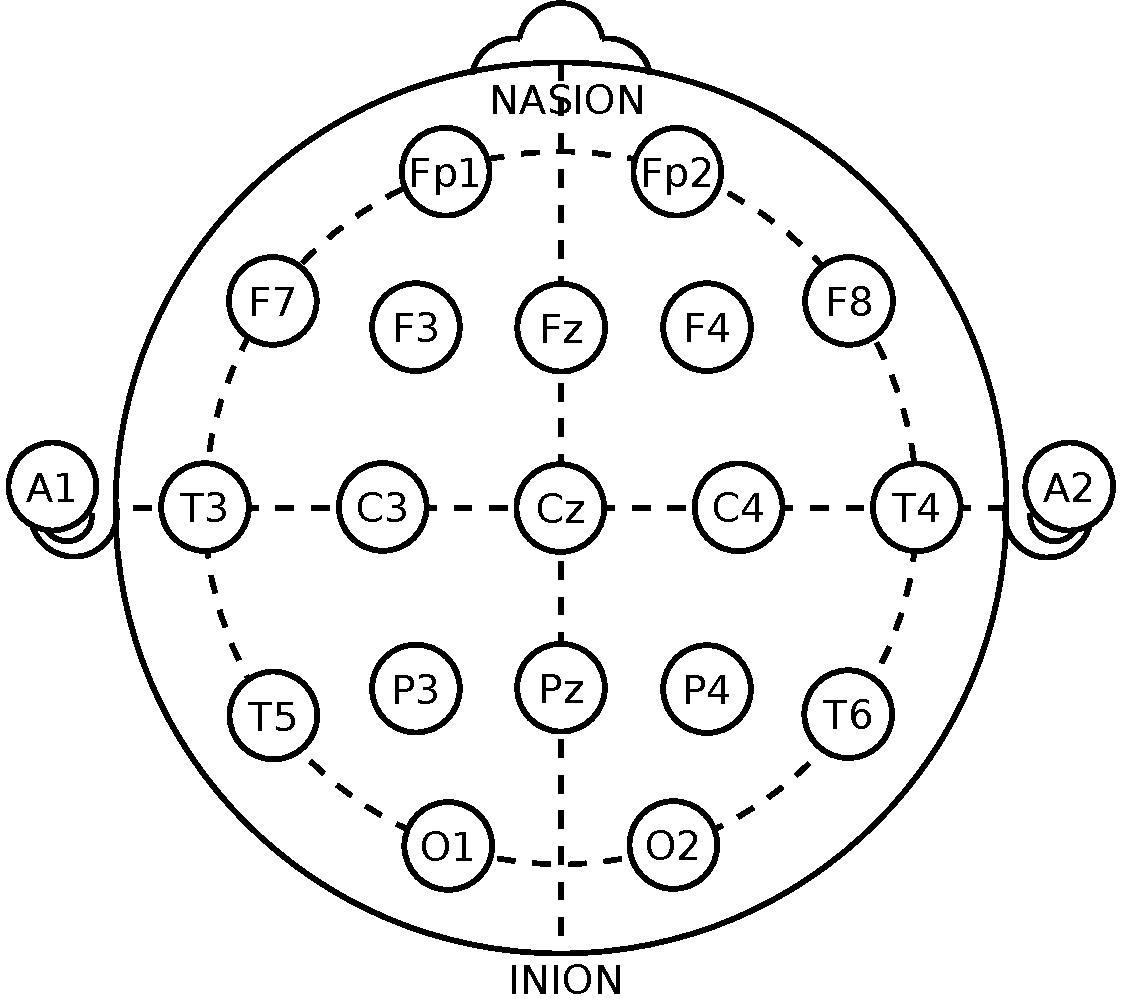
\includegraphics[height=0.45\linewidth]{pictures/tentwenty.pdf}
	\caption[Illustration of the $10$-$20$ system]{Illustration of the $10$-$20$ system used to place EEG electrodes provided by \citet{wiki:tentwenty}} \label{fig:tentwenty}
\end{figure}


Montages, voltage differences between certain probes, are used to extract information from these signals as opposed to the sole voltages sensed by the probes. Referential montages use the difference between a measuring electrode and a designated reference electrode. The reference electrode could be the ground which would mean the voltages sensed by the electrodes with respect to the ground can be used as the output of the EEG. In average reference montage, the outputs of all the electrodes are used as the reference voltage. Bipolar montages use the differences between two adjacent electrodes, e.g. F3 and C3 dubbed ``F3-C3'', as the output of the EEG. In Laplacian montages, the output is the voltage difference between an electrode and the average of the neighboring electrodes. 

A variety of different information can be extracted from these montages that can be used to classify the EEG activity. Frequency is one of these measurements. Rhythmic activity is considered to be constant in frequency, arhythmic activity is where no rhythms are present, dysrhythmic activity is a pattern that is rarely seen in healthy subjects. Frequency is also generally classified as delta, theta, alpha or beta waves. Delta waves have a frequency of $3$Hz or below, theta waves have frequencies between $3.5$Hz to $7.5$Hz, alpha waves have frequencies between $7.5$Hz and $13$Hz, and beta waves have frequencies above $14$Hz. Generally, only waves between $0$Hz and $70$Hz are considered since the rest of the signal is considered to be high-frequency noise in most cases and can be ignored.

The amplitude of these signals also tends to be useful. When a person is awake, beta waves usually dominate EEGs meaning that the average amplitude of the signals are small and the frequency is high. As a person starts to close their eyes, the average amplitude increases and the frequency starts to drop resulting in alpha waves. When a person starts to sleep, theta waves dominate, the average amplitude increases and the frequency decreases. Finally, in deep sleep, delta waves are observed in normal patients, the amplitude is generally large and the signal has very low frequencies. Therefore, we can logically deduce some things about the patient using amplitude and frequency together.  Heuristically say that if a person's EEG contains high frequencies and high amplitudes, they may be experiencing a seizure. 

However, such simplistic heuristics cannot always be used to extract useful information from patients. Therefore,  a professional \textit{or} an algorithm that considers the complexity of EEGs needs extract meaningful, diagnostic information.
\chapter{Related Work}
\label{relwork}

Deep metric learning is the task of using deep learning to learn a similarity metric using distance as a measure of similarity. Deep feature embedding learning is the task using deep learning to learn a set of features that aptly describes the original data and representing it in a vector space. Both of these tasks have been attempted many times before in a variety of different fields. 

\citet{facenet} used a DCNN trained with a triplet loss function to create an embedding space for facial recognition and facial similarity search. This model was trained to minimize the distance between an anchor and a positive and maximize the distance between an anchor and a negative. Mathematically,

\begin{equation}
  || f(x_{i}^{a} \ | \ \boldsymbol{\theta}) - f(x_{i}^{p} \ | \ \boldsymbol{\theta})||^2 + \alpha < || f(x_i^a \ | \ \boldsymbol{\theta}) - f(x_i^n \ | \ \boldsymbol{\theta}) ||^2
\end{equation}

\noindent
where $ \mathbf{\hat{y}} = f(X \ | \ \boldsymbol{\theta}) \in \mathbb{R}^d $ represents the computational graph, $a$ is the anchor, $p$ is the positive which is the same class as the anchor, $n$ is the negative which is not the same class as the anchor and $ \alpha$ is the margin parameter, a hyperparameter expressing the minimum distance between different clusters. Thus, the objective function becomes:  

\begin{equation}
  J = \sum_{i=1}^{N} \left[
  \norm{f(x_{i}^{a} \ | \ \boldsymbol{\theta}) - f(x_{i}^{p} \ | \ \boldsymbol{\theta})}^2
  - \norm{f(x_i^a \ | \ \boldsymbol{\theta}) - f(x_i^n \ | \ \boldsymbol{\theta}) }^2 + \alpha\right].
\end{equation}

\noindent
\citet{facenet} achieved $99.63\%$ accuracy on the Labeled Faces in the Wild dataset and a $95.12\%$ accuracy on the YouTube Faces DB dataset and it cut the error rate by $30\%$ compared to the previous state-of-the-art published by \citet{sun2014deeply}.

\citet{lifted_structure_embedding} provide a way of learning metrics through the use of what they describe as lifted structured feature embedding. Similar to \citet{facenet}, an input is fed into a neural network to produce a feature embedding. However, this scheme considers both the local and global structure of the embedding space. As opposed to triplet approach, this method does not require partitioning data into tuples in any manner. \citet{lifted_structure_embedding} find all the possible edges in a given mini-batch and describe whether they are similar or not using the Euclidean distance on the resulting embeddings and try to minimize a loss function based on those edges. They mathematically describe their loss function as the following: 

\begin{equation}
  \label{eq:lifted_structure_loss}
  \begin{gathered}
\tilde{J}_{i,j} = log \bigg( \sum_{(i,k) \in \mathcal{N}} \exp\{ \alpha - D_{i,k} \} + \sum_{(j,l) \in \mathcal{N}} \exp\{\alpha - D_{j, l}\} \bigg) + D_{i, j}
\\
J = \frac{1}{2 |\mathcal{P}|} \sum_{(i,j) \in \mathcal{P}} \max \Big( 0, \tilde{J}_{i,j}\Big)^2
  \end{gathered}
\end{equation}

\noindent
where $D_{i,k} = || f(\mathbf{X}_i) - f(\mathbf{X}_j)||^2$, $\alpha$ is the margin parameter, $\mathcal{P}$ is the set of positive pairs, $\mathcal{N}$ is the set of negative pairs, and $f$ is the network that produces the embeddings. This method achieved state of the art performance on standard datasets such as CUB200-2011, Cars196 and Stanford online products. However, this method represents a computational trade-off that may not necessary.

More ways of clustering raw data in the deep learning literature as those seen in \citet{jule, distknn, imgsimilarity} and \citet{errorprop}. However, little work has been done in trying to apply these methods to medical data to understand it better. 


% \citet{huang2015exclusive}

\citet{mlprepresentation} proposed Med2Vec which both learned distributed representations for medical codes and visits from a large EHR dataset, and also allowed for meaningful inerpretations which were confirmed by clinicians using a two-layer pereptron. They use information such as demographics, diagnosis information and prescription information to learn representations. Although the work done by \citet{mlprepresentation} works towards building a latent space for EMRs,  the model that they use is overly simplistic. Furthermore, it does not extract information directly from raw data. Hence, there is potential for loss of information.

\citet{goeg2015clustering} proposed a method for clustering models based on Systematized Nomenclature of Medicine - Clinical Terms (SNOMED CT) and used semantic similariy and aggregation techniques to hierarchically cluster EMRs. Similar to the work proposed by \citet{mlprepresentation}, their work relies on notes that were manually gathered by medical professionals and not the direct source of data itself. 

\citet{choi2016learning} proposed a method for learning low-dimensional representations of a wide range of concepts in medicine using claims data, which is more widely available to the public than annotations by medical professionals. They define  ``medical relatedness'' and  ``medical conceptual similarity'' by using current standards in medicine as established by the NDF-RT and the hierarchical ICD9 groups from CCS. They qualitatively evaluate their system and show that the top 5 neighbors for each input, sans duplicates, are medically related. Although their system works well, it still suffers from the same pitfall as the ones shown above. 

In fact, many more papers have attempted to cluster medical data and they have succeeded. However, they all seem to use only human annotations as input to their systems instead of both human annotations \textit{and} raw data. It is evident that there is a motion towards finding representations of medical records and medical data, however, the ways that are currently utilized are insubstantial due to the fact that they are using the analysis of data provided by medical professionals. Hence, this paper tries to fill this void by attempting to cluster raw EEG data in order to improve current methods of clustering EMRs. 

% \citet{yang2017frequency}


\chapter{Data and Resources}
\label{dataresources}

\section{Data}
\label{data}
The data for this study was derived from the Temple University Hospital's EEG corpus which includes over $30\text{,}000$ EEGs spanning the years from $2002$ to the present as described and provided by \citet{tuhwebsite}. The original data consists of raw European Data Format (EDF+\nomenclature{EDF+}{European Data Format}) files, a format commonly used for exchanging and storing multichannel biological and physical signals, and the corresponding labels for each of these files in LBL files. Both EDF files and the LBL files were stored in session folders with a single patient's data and doctors' notes on that patient's EEGs. There are a total of $339$ folders labeled from \verb+session1+ to \verb+session339+. The label files are interpretable by Temple University's publicly available Python script \cite{tuhwebsite}, which transforms the label files into a readable format.  Each channel is annotated as pertaining to one of six classes as described in \cref{tab:classes} with a granularity of one second. We assume that the data provided to us was time aligned correctly with the labels. For more details on the dataset see \citet{tuh}

\begin{table}[!ht]
	\captionsetup[table]{skip=10pt}
	\centering
	\caption[Set of classes]{Set of classes for the TUH EEG Corpus. After consulting \citet{harati2015improved}, it was determined that BCKG, ARTF and EYBL are noise-like signals, and the rest are seizure-like signals, i.e. indications of common events that occur in seizures. }
	\resizebox{\columnwidth}{!}{%
	\small
		\begin{tabular}{lm{10cm}l}
			\cmidrule{1-2}
			Code & Description                                  &                                                       \\ \cmidrule{1-2}
			BCKG & Background noise                             & \multirow{3}{*}{$\left. \vphantom{\begin{tabular}{c}3 \\3\\3\end{tabular}}\right\}$Noise-Like}\\
			ARTF & Artifacts                                    &                                                       \\
			EYBL & Eyeball movement                             &                                                       \\
			SPSW & Spikes \& sharp waves                        & \multirow{3}{*}{$\left. \vphantom{\begin{tabular}{c}3 \\3\\3\end{tabular}}\right\}$Seizure-Like}\\
			PLED & Periodic lateralized epileptiform discharges &                                                       \\
			GPED & Generalized periodic epileptiform discharges &                                                       \\\cmidrule{1-2}
		\end{tabular}
	}
	\label{tab:classes}
\end{table}

% \begin{table}[!ht]
% 	\captionsetup[table]{skip=10pt}
% 	\centering
% 	\caption[Set of classes]{Set of classes for the TUH EEG Corpus. After consulting \citet{harati2015improved}, it was determined that BCKG, ARTF and EYBL are noise-like signals, and the rest are seizure-like signals, i.e. indications of common events that occur in seizures. }
% 	\begin{tabular}{rL{10cm}}
% 		\toprule
% 		Code Name & Description                                  \\ \midrule
% 		BCKG     & Background noise                             \\
% 		ARTF     & Artifacts                                    \\
% 		EYBL     & Eyeball movement                             \\
% 		SPSW     & Spikes and sharp waves                       \\
% 		PLED     & Periodic lateralized epileptiform discharges \\
% 		GPED     & Generalized periodic epileptiform discharges \\\bottomrule
% 	\end{tabular}
% 	\label{tab:classes}
% \end{table}


The EDF files contain raw signals with different channels from electrodes placed in the standard $10$-$20$ system and were decoded using Python's MNE package. A total of $22$ montages were found in each label file. The power spectral density (PSD\nomenclature{PSD}{Power Spectral Density}) of the signal was visualized using the \verb+RawEDF.plot_psd()+ function. The bandwidth of the signals was between $0$ Hz to around $130$ Hz. It was revealed that the signals contained power line noise at $60$ Hz and $120$ Hz as seen in \cref{fig:psd}. 

\begin{figure}[!ht]
	\centering
	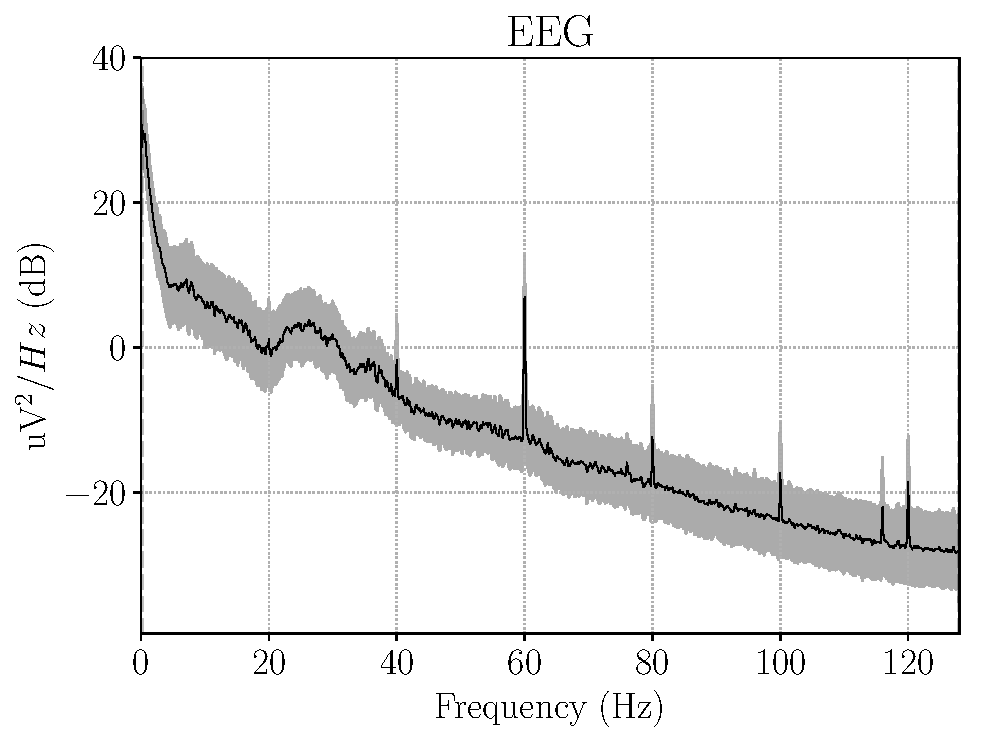
\includegraphics[width=0.7\linewidth]{pictures/psd.pdf}
	\caption[Power Spectral Density Plot of Raw Signals]{Power spectral density plot of raw signals using the MNE package}\label{fig:psd}  
\end{figure}

Hence, we apply notch filters at $60$ Hz and $120$ Hz to remove power line noise, and a band-pass filter with a $1$ Hz to $70$ Hz pass-band to remove any high-frequency noise as the bulk of the signal power was within this band. We apply the Short-Term Fourier Transform (STFT\nomenclature{STFT}{Short Term Fourier Transform}) provided by the MNE package with a window of $140$ samples and a stride of two samples which results in the spectrogram represented as a $71 \times 125$ tensor for each one-second window of the signal as shown in \cref{fig:stft}. 

\begin{figure}[!ht]
	\centering
	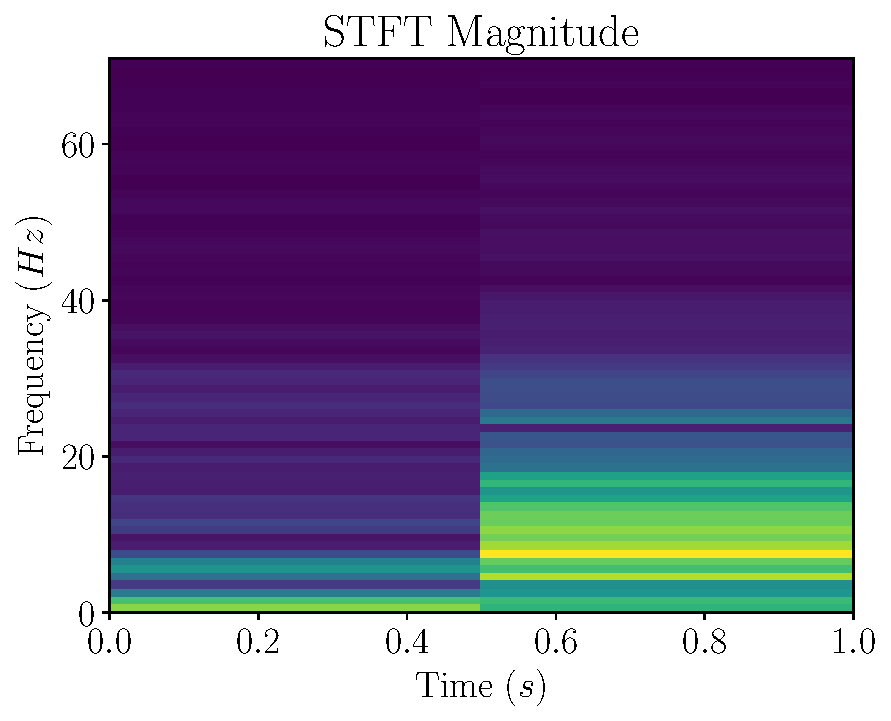
\includegraphics[width=0.65\linewidth]{pictures/plot21.pdf}
	\caption[Example of Spectrogram]{Spectrogram of a second of notch and band-pass filtered signal}\label{fig:stft}  
\end{figure}

Additionally, we globally normalize the signal power in order to standardize the input to the system that we designed and only use the real part of the spectrogram data. The raw time-domain data was not utilized in this experiment because the literature \cite{eegs_info, eeg_info2, mayo_eegs} on EEGs indicated that the frequency domain is what contains data that is useful for our purpose.

We did not use the spatial information implicitly provided to us by the $10$-$20$ system's spatial structure. This decision was made because the resulting tensor would have become a $22 \times 71 \times 125$ tensor of values and the amount of time taken to process this tensor would have been longer than the time taken to process a $71 \times 125$ tensor. Furthermore, even if it were computationally possible for us to process the larger tensor for each second of signal, there was no possible way to consistently label the tensor as each montage was labeled independently of the others. Hence, there was no possible way to consistently label all $22$ montages with a single label. As a result, we only used a single channel's input as opposed to all $22$ channels' inputs. 

We also realized that the dataset is highly imbalanced. More than $80\%$ of the data was labeled as noise-like signals. Since we were looking for anomalies in the dataset, it was necessary to use stratified sampling to help compensate for this imbalance which may result in imbalanced training. We split the $71 \times 125$ tensors into mutually exclusive training and validation sets. Each set is disjoint in both patient and sample acquisition, i.e. no single patient appears in both sets and no two windows from a single acquisition appear in both sets. We follow an $85/15\%$ split for the training/validation set. Due to the large nature of the training set in this situation and the impossibility of training on every triplet possible, a random set of triplets were selected for each training iteration. 

\section{Resources}


\subsection*{Tensorflow}

Tensorflow and TF-Slim, as described by \citet{tensorflow} and \citet{tfslim},  are frameworks which provided a way to build scalable, computational graphs for machine learning. Tensorflow's use of automatic differentiation, as described by \citet{autodiff}, allowed for precise calculations of gradients for networks without floating-point errors. Furthermore, automatic differentiation also helped in this project since the loss function depended on multiple example data points, i.e. the anchor, the positive and the negative,  as opposed to a single example data point. TF-Slim's implementation of commonly used computational graph layers (e.g. convolutional layers) helped us define the network without explicitly defining and coding weight matrices. 

\subsection*{SciKit Learn}
SciKit Learn is a Python module developed by \citet{sklearn} that provided implementations of common machine learning algorithms and some commonly used accessory functions. In particular, it provided us the k-NN algorithm used throughout the paper to classify validation signals, the confusion matrix calculation function used to analyze our validation results, and the t-SNE reduction algorithm used to analyze the high dimensional latent space in a reduced, 2-dimensional space. SciKit Learn was also built with NumPy and matplotlib, and was easily compatible with the rest of our source code. 

\subsection*{MNE Package}

The MNE package is a Python module developed by \citet{mne} that provided implementations for manipulating biological signal data. It has functions necessary to read, analyze, filter and convert raw data in EDF files to NumPy arrays. These functions allowed us to refine the data instead of processing the raw, time-domain signal.
\chapter{Experiment and Results}
\label{expres}

After a considerable amount of research in clustering and metric learning, we chose triplet loss as our method of approaching the problem. Triplet loss is well-established, simple and effective when it comes to learning a latent space. Other methods such as the one proposed by \citet{lifted_structure_embedding} were overly complicated, especially given the size of our dataset. Triplet loss was relatively easy to implement considering how we organized the transformed data and so, a network trained on triplet loss was the natural choice for this experiment. 

\section{Initial Experiments}

Initially, we did not know whether this method would work on the STFT transformed signals as described in \cref{data} and we needed a simple way to test out the concept. Hence, to learn the latent space, we needed to start with a relatively simple network. 

Although the network's architecture was not a priority since this was only a test run of the concept, CNNs were considered from the very beginning since they perform very well in image and video processing tasks as mentioned in \cref{cnns}. Spectrograms inherently look like images as we saw in \cref{fig:stft}. Since we are using spectrograms of the EEG signals as the input, it made sense to use CNNs. Secondly, we assumed that the labels for each second of each channel of original signal were properly time-aligned in the time domain. In case that this assumption is invalid, CNNs still can perform better than other types of networks. CNNs tend to learn the patterns in the spectrogram even if they were not time-aligned since they learn shift-invariant features. Hence, an important feature that starts in the first interval of the spectrogram may still be recognized even if it starts sixty intervals later.

\begin{table}[!ht]
	\centering
	\small
	\caption{Network architecture for CNN}
	\begin{tabular}{rllc}
		\toprule
		Layer  & Input                       & Output                      & Kernel         \\ \midrule
		conv1  & $ 71 \times 125 \times 1 $  & $ 71 \times 125 \times 32 $ & $ 4 \times 4 $ \\
		pool1  & $ 71 \times 125 \times 32 $ & $ 35 \times 62 \times 32 $  & $ 3 \times 3 $ \\
		conv2  & $ 35 \times 62 \times 32  $ & $ 35 \times 62 \times 64 $  & $ 5 \times 5 $ \\
		pool2  & $ 35 \times 62 \times 64 $  & $17 \times 30 \times 64$    & $ 2 \times 2 $ \\
		fc1    & $17 \times 30 \times 64$    & $ 256          $            & N/A            \\
		fc2    & $ 256 $                     & $ 128 $                     & N/A            \\
		output & $ 128 $                     & $ 64   $                    & N/A            \\ \bottomrule
	\end{tabular}
	\label{tab:network}
\end{table}

Eventually, we built our initial model described in \cref{tab:network} in TensorFlow as described by \citet{tensorflow}. The  code in \cref{initial_model_code} was used to build the network described. We trained the initial model on a Lenovo Y700 laptop running Ubuntu $16.06$ LTS with an Intel Core i7-6700HQ CPU running at $2.60$ GHz, $8$ GB of RAM and no discrete graphics card for Tensorflow's CUDA acceleration capabilities. 

In our first attempt, the loss function converged to values very close to zero within the first few iterations. After stepping through the code, we discovered that the input data values were all in the $10^{-5}$ order of magnitude. As a result, the network was discovering a trivial solution that would satisfy the loss function but at the same time not solve the problem at hand. In order to avoid this, we amplified the input data by multiplying all inputs to the network by $10^4$. The network started to train normally and we noticed that the network's loss started to decrease in the expected exponential manner. Semi-hard or hard triplets were chosen at run-time to train the network. Any ``soft'' triplets were skipped until semi-hard or hard triplets were found since they do not contribute to the learning of the space. 

\subsection{Hyperparameter Selection}

Initially, we had selected random hyperparameters for the network. Once we realized that the network started to train as we intended it to, we needed to select the hyperparameters the learning rate, $\eta$, the margin parameter, $\alpha$, the regularization strength, $\lambda$ and the output dimension, $d$. More attention was given to $\eta$ since we wanted the network to converge fast but not oscillate before reaching convergence. Despite using the Adam optimizer, the oscillation described in \cref{paramsmodeling} can still occur due to small, deep valleys in the hypersurface created by the loss function. In most experiments that we've seen, $\lambda$ is typically a magnitude below the learning rate. We continued that convention and selected $\eta = 10^{-3}$ and $\lambda=10^{-4}$. Regularization was not necessarily important at this point so not much attention was given to $\lambda$.  The rest of the parameters were chosen to be ``nice'' numbers and were $\alpha = 1.0$, and $d=128$.  

We attempted running the network for a hundred thousand iterations. However, we noticed that after fifty thousand iterations, the triplet mining process was slowed down because the script found it difficult to find semi-hard or hard triplets. At one point, we observed that nearly two hundred thousand triplets were skipped due to their soft nature. Due to this phenomenon, we hypothesized that the network had started to converge at around sixty thousand iterations and decided that it was no longer needed to train. After that point, this particular network architecture was trained for sixty thousand iterations and the data pool was changed every ten thousand iterations to help the script find more semi-hard or hard triplets. This alleviated the stalling nature of triplet mining. 

\subsection{Measuring Performance}

Although the loss was decreasing as expected, we needed a way of validating whether the space that we anticipated was actually forming. One way to do this was to follow the advice given by \citet{facenet} and use a k-NN classifier to quantify the quality of the embedding space produced. Assuming that the data provided was classified correctly, we run some training data through the network to find the embeddings of those samples. We then populate the k-NN space with those embeddings. New embeddings produced from the validation set are introduced to the k-NN algorithm and classified. Theoretically, if the embedding space develops distinct clusters based on the classes, it would classify the validation signals with a relatively high overall accuracy since the validation set's embeddings would be near the cluster.  

We used SciKit Learn's implementation of the k-NN classifier to apply the test described. The default value of the number of neighbors, $k=5$, was used to classify the validation embeddings produced. This test results were accurate 80\% of the time. At this point, we were not using stratified sampling to adjust for the data imbalance. Hence, we assumed that most of the data that was classified incorrectly were originating from classes with low numbers of samples points. It was clear that the experiment was a success and our initial hypothesis that triplet loss can be used learn a latent space for EEGs was valid since the resulting accuracy was relatively high considering that we only used a very simple, two-layer CNN.

\subsection{Error in Dataset Organization}

Unfortunately, the success that we experienced with the initial network was not long-lasting. When we explored the various sources of errors in the experiment, it was obvious that the amount of time used to train the network and the overall accuracy of the network was qualitatively low and high, respectively. Therefore, we tried to inspect the code used so far for any possible errors that we may have introduced. We discovered that the data used to train the network was organized in a way such that the different classes of data were easily split, but the patients, i.e. the different sessions, were not. Therefore, when training, we were implicitly training and validating on a portion of the training set which was already seen. 

Our goal was to make this system general so that the system can detect the presence of any of the six signals in any patient, not only for the patients provided in the dataset. Hence, it was necessary for us to reorganize the data so that it was split by session \textit{and} class. We split the dataset again so that sessions from \verb+session1+ until \verb+session300+ were used as training data and the rest of the sessions were used as testing data while retaining all information about the signal including session, type of signal and time of the signal in the session. This ensured that the training set and the validation set were truly mutually exclusive. Furthermore, the new method of organization helped in conducting analysis of files with seizure-like signals and files with noise-like signals which will be discussed in \cref{analysis}.

\section{DCNN with Triplet Loss}

As discussed in \cref{bias_variance_tradeoff}, it is generally easier to cut down a model by using regularization than it is to increase the complexity of a model. Since the concept of using triplet loss to train a CNN for clustering EEG signals was validated, it made sense to proceed to the next step and experimentally increase the complexity of the network. The next logical step from two-layer CNN was to make a DCNN that used multiple layers of convolution to learn more complex shift-invariant features.

We continued the same convolutional layer followed by maxpool layer pattern with a fully connected layer at the end, as seen in the initial network shown in \cref{tab:network}. Our new network, specified in \cref{tab:dcnn}, consisted of five convolutional layers each followed by a maxpool layer. We built the network using Tensorflow again and trained the model on a server with Intel Xeon ES-2620 24-core CPU with each core at $2.10$ GHz, $128$ GB of RAM and five Nvidia GeForce Titan X GPUs with $12$ GiB of video memory for Tensorflow's GPU acceleration.

\begin{table}[!ht]
	\centering
	\small
	\caption{Network architecture for simple CNN}
	\begin{tabular}{rllc}
		\toprule
		Layer    & Input                     & Output                    & Kernel       \\ \midrule
		conv1    & $71 \times 125 \times 1$  & $71 \times 125 \times 32$ & $5 \times 5$ \\
		maxpool1 & $71 \times 125 \times 32$ & $34 \times 61 \times 32$  & $5 \times 5$ \\
		conv2    & $34 \times 61 \times 32$  & $34 \times 61 \times 64$  & $3 \times 3$ \\
		maxpool2 & $34 \times 61 \times 64$  & $16 \times 30 \times 64$  & $3 \times 3$ \\
		conv3    & $16 \times 30 \times 64$  & $16 \times 30 \times 128$ & $2 \times 2$ \\
		maxpool3 & $16 \times 30 \times 128$ & $8 \times 15 \times 128$  & $2 \times 2$ \\
		conv4    & $8 \times 15 \times 128$  & $8 \times 15 \times 256$  & $1 \times 1$ \\
		maxpool4 & $8 \times 15 \times 256$  & $4 \times 7 \times 256$   & $2 \times 2$ \\
		conv5    & $4 \times 7 \times 256$   & $4 \times 7 \times 1024$  & $4 \times 4$ \\
		maxpool5 & $4 \times 7 \times 1024$  & $1 \times 2 \times 1024$  & $4 \times 4$ \\
		flatten  & $1 \times 2 \times 1024$  & 2048                      & N/A          \\
		fc1      & 2048                      & 1024                      & N/A          \\
		fc2      & 1024                      & 512                       & N/A          \\
		fc3      & 512                       & 256                       & N/A          \\
		output   & 256                       & 64                        & N/A          \\ \bottomrule
	\end{tabular}
	\label{tab:dcnn}
\end{table}


\subsection{Hyperparameter Selection}
The architecture of the network itself can be varied and may be considered a hyperparameter by itself. We can vary the number of layers, the number of neurons in each layer, the convolutional kernel size, the activation functions, parameter initialization methods and so on. However, this is something that is developed with experience in the field. There are ways to make some of those hyperparameters learnable. For example, the work done by \citet{inception} allows a single convolutional layer to have variable kernel sizes. When using backpropagation, the network can learn which kernels are used and how much they are used in determining the final output. \citet{prelu} work on the parametrization of the ReLU activation function in order to help learn what type of activation function is optimal for a given task. However, such ways of improving the architecture are outside of the scope of this thesis and introduces more issues that increase the overall complexity of the network. 

Following the results of the initial experiment, we started to train the new network with the same hyperparameters as the network shown in \cref{tab:network} and decided to pivot on the hyperparameters as necessary in order to find the best model that both generalizes well to the validation set and forms a relatively compressed latent space. We did a manual grid search on a particular range for each of the hyperparameters, $\eta$, $\alpha$, $\lambda$ and $d$. We cross-validated the networks' ability to infer what new signals might be by using the validation set that we had set aside. After training the network and cross-validating, it was found that $\eta=10^{-4}$ , $\alpha=0.5$, $\lambda = 10^{-3}$ and $d=64$ led to the best results. 

\subsection{Measuring Performance}

We still used k-NN classification accuracy as a measure of the quality of the latent space produced. However, in order to make sure that the classification was being done correctly, we elected to change the number of neighbors that the k-NN algorithm used to a higher value. Increasing $k$ effectively smoothens the decision boundary since the algorithm uses more neighbors to make its decisions. After experimentally increasing the number of neighbors the algorithm considered to make the classification decision in the latent space, we chose $k=31$ as it had the highest level of accuracy and completed the task quickly with the amount of available memory.  With those hyperparameters, we achieved a validation accuracy of $60.4\%$. The confusion matrix for that iteration of cross-validation is shown in \cref{fig:dcnnlarge}. 

\begin{figure}[!ht]
	\centering
	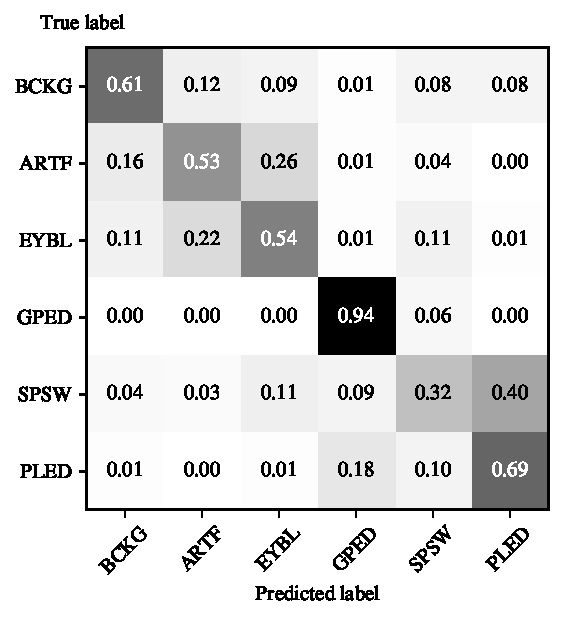
\includegraphics[width=0.7\linewidth]{pictures/conf_mat_exp.pdf}
	\caption[Confusion matrix for the DCNN clustering network]{Confusion matrix for the DCNN clustering network with $\alpha = 0.5$, $\eta = 10^{-5}$ after $105$k iterations, and an accuracy of $60.4\%$ with 31-NN classification}\label{fig:dcnnlarge}
\end{figure}

The classification accuracy provides a numerical value which could be used as a measure of the quality of the embedding that our system produces. However, this does not necessarily provide us information on whether clusters are forming, which is what we were hoping would happen from the beginning. In order to test how well the network was doing in clustering signals based on similarity, we decided to apply t-distributed stochastic neighbor embedding  (t-SNE\nomenclature{t-SNE}{t-Distributed Stochastic Neighbor Embedding}) which is an algorithm that reduces the dimensionality of high dimensional data. Although this algorithm reduces the dimensionality, the overall structure of the latent space remains the same as the structure of the $d$-dimensional latent space. If clusters exist in the t-SNE plot, it would mean that the same clusters are highly likely to exist in the $d$-dimensional latent space. Hence, we used t-SNE to visualize the $64$ dimension latent space in $2$D. The t-SNE reduced two dimensional embedding after $5$k iterations is shown in \cref{fig:tsne_start} and the same after $105$k iterations is shown in \cref{fig:tsne}. 

\begin{figure}[!ht]
	\centering
	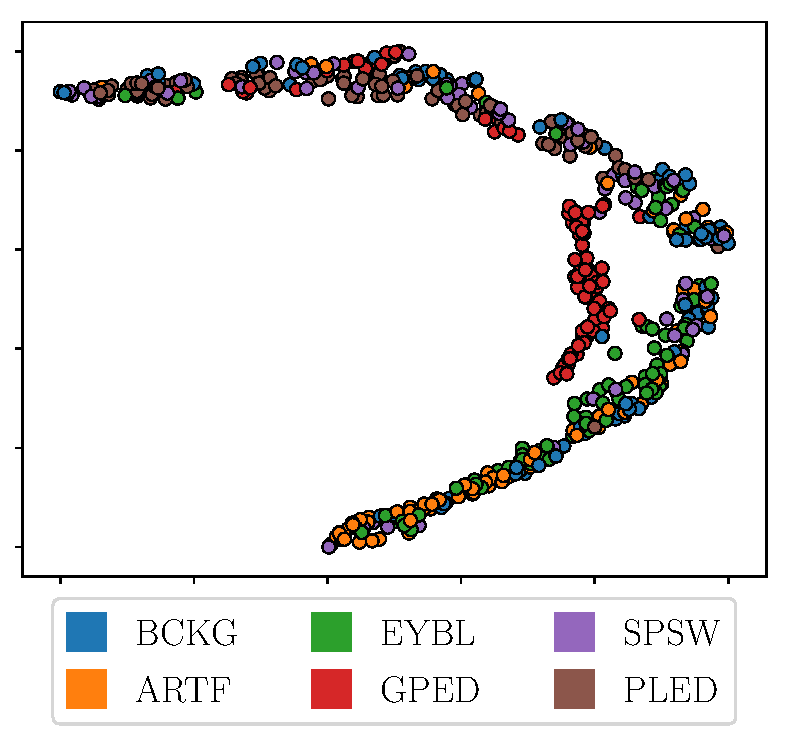
\includegraphics[width=0.65\linewidth]{pictures/tsne_plot_start.pdf}
	\caption[t-SNE visualization after $5$k iterations]{t-SNE reduced 2D visualization  of validation set for the DCNN clustering network after five thousand iterations with $\alpha = 0.5$, $\eta = 10^{-5}$ after $5$k iterations, and an accuracy of $26.6\%$ with 31-NN classification after EEG signal was passed through the DCNN clustering network}\label{fig:tsne_start}  
\end{figure}


\begin{figure}[!ht]
	\centering
	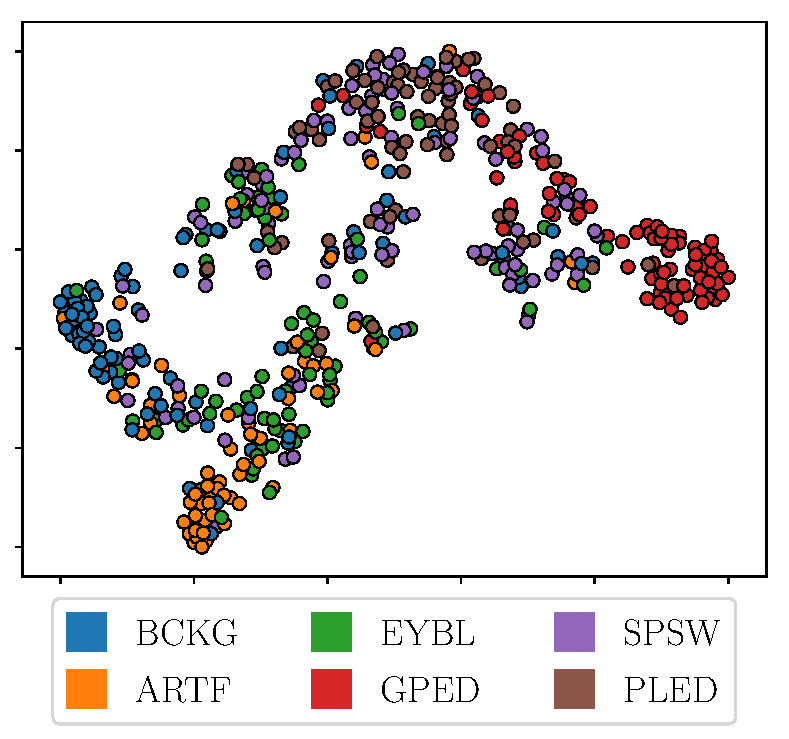
\includegraphics[width=0.65\linewidth]{pictures/tsne_plot.pdf}
	\caption[t-SNE visualization after $105$k iterations]{t-SNE reduced 2D visualization  of validation set for the DCNN clustering network with $\alpha = 0.5$, $\eta = 10^{-5}$ after $105$k iterations, and an accuracy of $60.4\%$ with 31-NN classification after EEG signal was passed through the DCNN clustering network}\label{fig:tsne}  
\end{figure}

We can see a clear difference of the t-SNE embedding after $100$k iterations. Initially, \cref{fig:tsne_start} shows that the GPED signal is separating out from the crescent in the middle but, the rest of the classes are far off from forming their own clusters and are mixed together. However, \cref{fig:tsne} shows that the clusters are forming even in a $2$-dimensional space.  GPED, BCKG and ARTF have clearly split away from each other and have formed their own clusters. 

We see a lot of qualitative correlation between the confusion matrix in \cref{fig:dcnnlarge} and t-SNE plot in \cref{fig:tsne}. For example, according to the confusion matrix GPED was classified correctly $94\%$ of the times that it was encountered in the validation set. This makes sense since the t-SNE plot shows a large cluster of GPED signals. Hence, we can conclude that the clustering algorithm is probably working well because of the amount of qualitative correlation between the t-SNE plot and the confusion matrix.


\subsection{Comparison with a DCNN Classifier}
Another way to measure the performance of the clustering network is to compare it with a baseline algorithm. Since we are evaluating the performance of a neural network as a method of clustering EEG signals, we would like to find out how the same architecture as a classifier would perform so that we could compare their performance. In order to keep the same architecture so that we are confident that the architecture would not make a difference, we just add a fully-connected layer to the network shown in \cref{tab:dcnn} as a classification layer with a softmax activation without changing anything else and train the network on the softmax cross-entropy loss function used in neural network classifiers. We use the same exact hyperparameters as we use in training the clustering network and achieve a validation accuracy of $50.2\%$. The confusion matrix for the results of this network is shown in \cref{fig:dcnnclasslarge}. 

\begin{figure}[!ht]
	\centering
	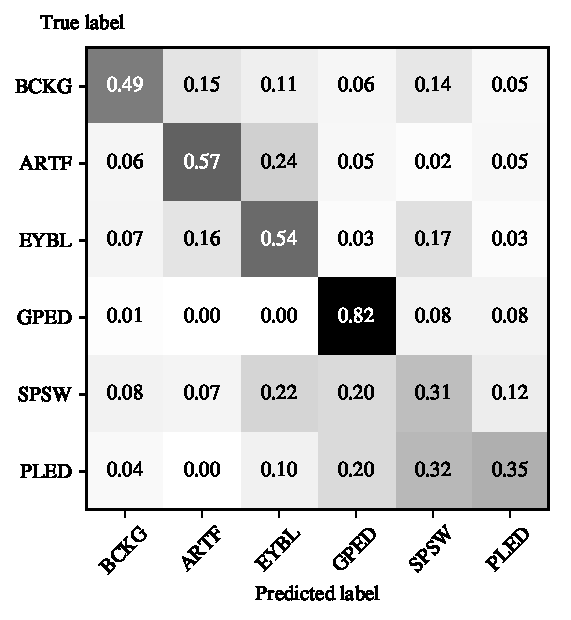
\includegraphics[width=0.55\linewidth]{pictures/conf_mat_baseline.pdf}
	\caption[Confusion matrix for the baseline DCNN classifier]{Confusion matrix for the baseline DCNN classifier with the same hyperparameters as \cref{fig:dcnnlarge} after 200k iterations and an accuracy of $50.2\%$ with $31$-NN classification}\label{fig:dcnnclasslarge}  
\end{figure}

These results were perplexing. A classifier is particularly trained on the task of discriminating between different classes whereas our clustering network is trained on the triplet loss which hoped to group similar signals together. It was surprising that a network trained to classify did not do better than the network that was trained to cluster. These results suggest that it may actually better to use the triplet loss in any situation since it provides more information about the original data, can work with any number of classes and possibly detect new classes once trained, and still perform better than the DCNN on a classification task. 

Furthermore, it is likely that this phenomenon occurred directly due to the differences in loss functions since each network had nearly identical architectural forms. The features learned by the DCNN trained on the triplet loss and the features learned by the penultimate layer in the DCNN classifier are probably different because of the difference in the way the networks are trained.

\subsection{Binary Classification Using the Latent Space}

We were curious as to how well our system would work if we only used it to classify a signal as either a seizure-like signal or noise-like signal.  We considered BCKG, EYBL and ARTF to be noise-like signals, and SPSW, GPED and PLED to be seizure-like signals as shown in \cref{tab:classes}. We can pose this as a k-NN classification problem since our network has already been trained. We found the binary classification confusion matrix as shown in \cref{fig:conf_mat_exp_pooled} and found the overall accuracy to be $90.2\%$.

\begin{figure}[!ht]
	\centering
	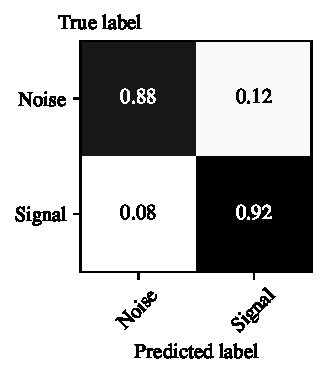
\includegraphics[width=0.425\linewidth]{pictures/conf_mat_exp_pooled.pdf}
	\caption[Binary Confusion Matrix for  the DCNN Clustering Network]{Binary confusion matrix for the DCNN clustering network with $\alpha = 0.5$, $\eta = 10^{-5}$ after $105$k iterations, and an accuracy of $90.2\%$ with 31-NN classifier}\label{fig:conf_mat_exp_pooled}
\end{figure}

\begin{figure}[!ht]
	\centering
	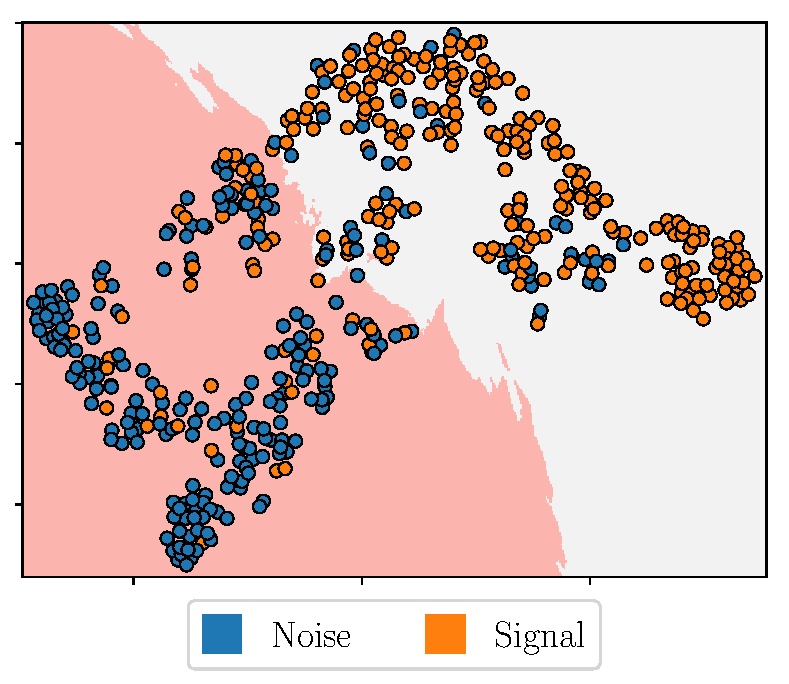
\includegraphics[width=0.7\linewidth]{pictures/tsne_plot_binary.pdf}
	\caption[k-NN Binary Decision Boundary on t-SNE Reduced Embedding]{k-NN classifier decision boundary for t-SNE reduced 2D visualization of validation set for the DCNN clustering network after five thousand iterations with $\alpha = 0.5$, $\eta = 10^{-5}$ after $105$k iterations and a 31-NN classifier}\label{fig:tsne_plot_binary}  
\end{figure}

Modifying the t-SNE to label seizure-like signals and noise-like signals, and plotting the decision boundary of a k-NN classifier as shown in \cref{fig:tsne_plot_binary} demonstrates that there is a boundary that separates seizure-like signal from noise-like signal clearly. Even though we trained on all types of triplets (e.g. PLED-PLED-GPED, GPED-GPED-BCKG etc.), we still found a clean separation between seizure-like signals and noise-like signals. This phenomena demonstrates that not only are the set of triplet classes that we train on separating, but their super classes, i.e. the general signal types, are separating which can possibly lead to a better, hierarchical taxonomy. 

\section{Analysis on Seizure-Like \& Noise-Like Files}
\label{analysis}
Although our network has done quite well on a rather noisy dataset, a thorough error analysis is certainly the most important step in order to determine how to pivot. In order to conduct this error analysis, we look at how the network performs on subsets of the data and try to discover any patterns or explanations that might help us improve the network in order to get better results. We split the data into the following three subsets: 
\begin{itemize}
	\setlength\itemsep{1mm}
	\item sessions without seizure-like signals
	\item sessions with seizure-like signals
	\item sessions with seizure-like signals considering only seizure-like signals
\end{itemize}
   
We were able to separate the different signals based on their original session and what types of signals existed in that session. Every time we compute a confusion matrix for validating the network on the stratified sampled dataset, we also compute a confusion matrix for a stratified sampled subset of the dataset for each of the above categories. In doing so, we obtain the following results. 

\begin{figure}[!ht]
	\centering
	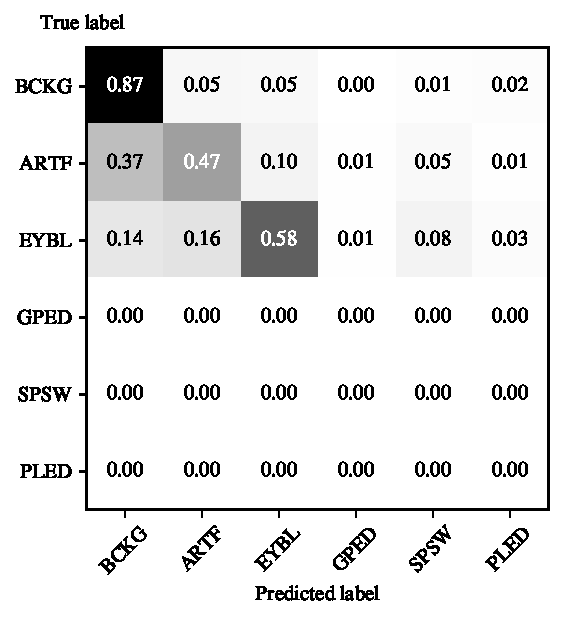
\includegraphics[width=0.7\linewidth]{pictures/conf_mat_exp_without_seizure.pdf}
	\caption[Confusion Matrix on Sessions without Seizure-Like Signals]{Confusion matrix of DCNN clustering network on files without seizures resulting in an accuracy of $64.6\%$ with $\alpha = 0.5$, $\eta = 10^{-5}$ after $105$k iterations and a 31-NN classifier}\label{fig:conf_mat_exp_without_seizure}  
\end{figure}

The confusion matrix shown in \cref{fig:conf_mat_exp_without_seizure} is on the data from sessions that do not contain any seizure-like signals. These sessions only contain BCKG, ARTF and EYBL signals. Hence, the bottom half of the confusion matrix is empty. The right half of the confusion matrix is not completely empty because the DCNN along with the k-NN classifier still predicts some of these signals to be GPED, SPSW or PLED since the network is still trained on the training set which contains all the classes. These incorrect predictions are expected to occur due to various sources of natural background noise, and incorrect true labels or shared characteristics that are closer to seizure-like signals as opposed to noise-like signals. This results in a $64.6\%$ overall accuracy after $105$k iterations.

\begin{figure}[!ht]
	\centering
	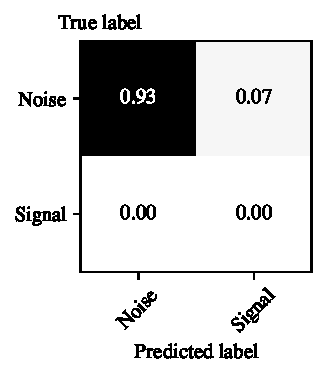
\includegraphics[width=0.425\linewidth]{pictures/conf_mat_exp_without_seizure_pooled.pdf}
	\caption[Binary Confusion Matrix on Sessions without Seizure-Like Signals]{Binary classification confusion matrix of DCNN clustering network on files without seizures resulting in a binary accuracy of $93.0\%$ with $\alpha = 0.5$, $\eta = 10^{-5}$ after $105$k iterations and a 31-NN classifier}\label{fig:conf_mat_exp_without_seizure_pooled}  
\end{figure}

As we had done before, we had also made a binary confusion matrix as well. Just like the confusion matrix presented in \cref{fig:conf_mat_exp_without_seizure}, the bottom half of the confusion matrix is empty and the top-right of the confusion matrix is not empty. The system achieved a $93\%$ accuracy in detecting that a second of signal is noise-like and not a seizure-like signal. In other words, given only noise-like signals, we are able to classify 93\% of those signals as noise-like signals using our system and the remaining 7\% as not noise-like (i.e. seizure-like) signals. 

The confusion matrix in \cref{fig:conf_mat_exp_with_seizure} is on sessions that contain seizure-like signals. Sessions that contain seizure-like signals also contain noise-like signals since the entire session is not full of seizure-like signals. Therefore, all the types of signals are present in the confusion matrix. However, these sessions are mutually exclusive from the sessions that we looked at in \cref{fig:conf_mat_exp_without_seizure} since those sessions do not contain any seizure-like signals at all. When looking at sessions that contain seizure-like signals, we obtained an overall accuracy of $56\%$ after $105$k iterations.

\begin{figure}[!ht]
	\centering
	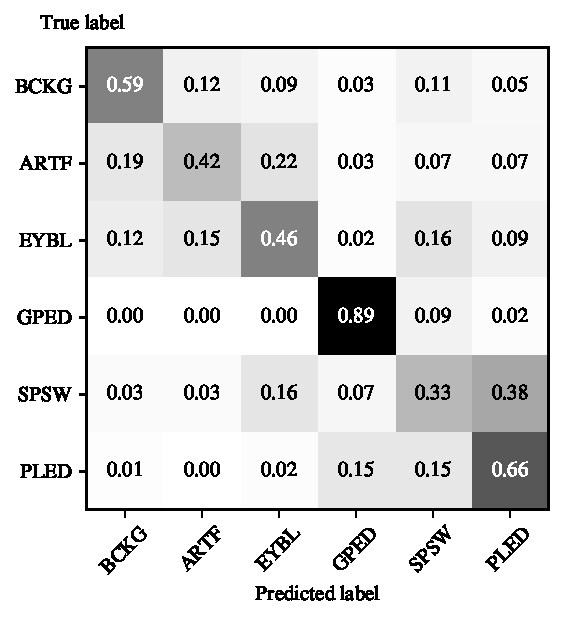
\includegraphics[width=0.7\linewidth]{pictures/conf_mat_exp_with_seizure.pdf}
	\caption[Confusion Matrix on Sessions with Seizure-Like Signals]{Confusion matrix of DCNN clustering network on files with seizures resulting in an accuracy of $56.0\%$ with $\alpha = 0.5$, $\eta = 10^{-5}$ after $105$k iterations and a 31-NN classifier}\label{fig:conf_mat_exp_with_seizure}  
\end{figure}

As before, we also constructed a binary classification confusion matrix. In this case, given that the session contains a seizure, we are able to classify the signal as seizure-like or noise-like with an accuracy of 85\%. The noise-like signals were detected correctly 78\% of the time and the seizure-like signals were detected correctly 91\% of the time. 


\begin{figure}[!ht]
	\centering
	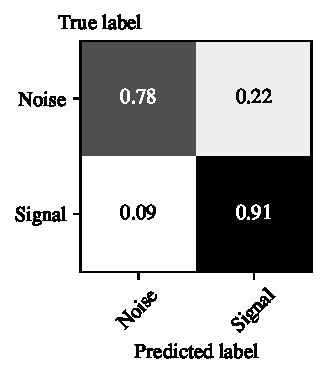
\includegraphics[width=0.425\linewidth]{pictures/conf_mat_exp_with_seizure_pooled.pdf}
	\caption[Binary Confusion Matrix on Sessions with Seizure-Like Signals]{Confusion matrix of DCNN clustering network on files with seizures resulting in an accuracy of $85.0\%$ with $\alpha = 0.5$, $\eta = 10^{-5}$ after $105$k iterations and a 31-NN classifier}\label{fig:conf_mat_exp_with_seizure_pooled}  
\end{figure}

Finally, the confusion matrix in \cref{fig:conf_mat_exp_with_only_seizure} is on sessions that contain seizure-like signals excluding noise-like signals to explore how the system performs on just signals that have seizures (i.e. GPED, SPSW, PLED). This is why the top half of the confusion matrix is empty and we see that most of the predictions are within the bottom right square of the confusion matrix, which is what we expected. Note that the signals that were tested to produce this confusion matrix are not necessarily mutually exclusive from the signals that we tested in \cref{fig:conf_mat_exp_with_seizure} since the signals used to form that confusion matrix were the ones that contained seizures. The experiment results in an overall validation accuracy of $60.4\%$ after $105$k iterations. We also see that a lot of the SPSW are being classified as PLED. This is likely because of the high similarity between PLED and SPSW.

\begin{figure}[!ht]
	\centering
	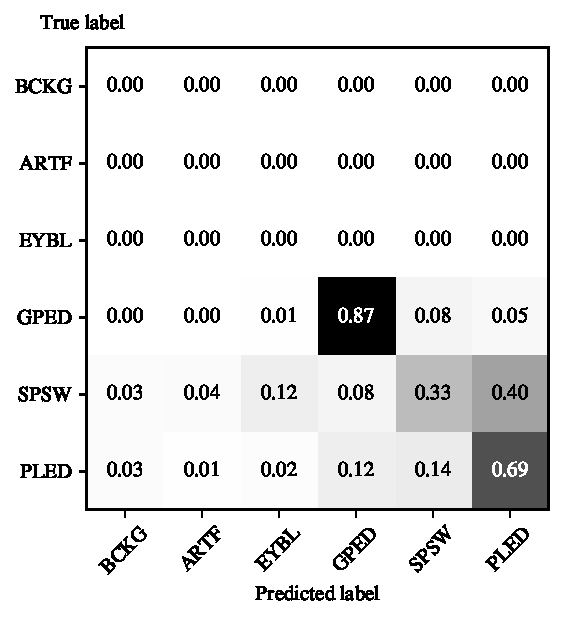
\includegraphics[width=0.7\linewidth]{pictures/conf_mat_exp_with_only_seizure.pdf}
	\caption[Confusion Matrix on Sessions with only Seizure-Like Signals]{Confusion matrix of DCNN clustering network on files with ONLY seizure signals resulting in an accuracy of $63.0\%$ with $\alpha = 0.5$, $\eta = 10^{-5}$ after $105$k iterations and a 31-NN classifier}\label{fig:conf_mat_exp_with_only_seizure}  
\end{figure}

\begin{figure}[!ht]
	\centering
	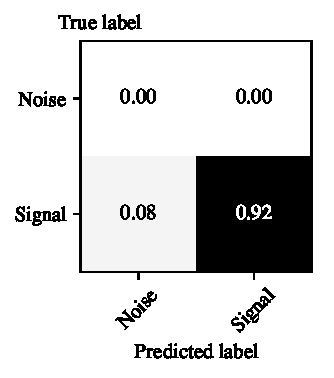
\includegraphics[width=0.425\linewidth]{pictures/conf_mat_exp_with_only_seizure_pooled.pdf}
	\caption[Binary Confusion Matrix on Sessions with only Seizure-Like Signals]{Confusion matrix of DCNN clustering network on files with ONLY seizure signals resulting in an accuracy of $91.8\%$ with $\alpha = 0.5$, $\eta = 10^{-5}$ after $105$k iterations and a 31-NN classifier}\label{fig:conf_mat_exp_with_only_seizure_pooled}  
\end{figure}

Similar to the last experiment, we also generated a binary classification confusion matrix. Given that the session contains a seizure and we are only looking at a seizure-like signal in that particular session, we are able to observe that the signal presented to the system is seizure-like 92\% of the time and mis-classified the signal as noise 8\% of the time. 

In doing the analysis on the subsets of the validation set, it is revealed that most of the error in attempting to recognize a signal as a one of the types of seizure-like signals arises because the signal is classified as one of the other types of seizure-like signals. For example, if a signal with PLED as the true label is presented to the system and the system makes an error in predicting the label of the signal, it is likely for the prediction to be SPSW or GPED as opposed to the noise-like signals. A possible reason for this phenomena may be because the given signal is more similar to SPSW or GPED. This phenomena is acceptable because the system is expected to cluster and place similar signals near each other. Logically this makes sense since the seizure-like signals are expected to be more similar to each other than noise-like signals. The binary confusion matrices support this observation since it has a high true positive rate and a high true negative rate. 

Another common error that was seen in the various confusion matrices was the relatively high false classification rate of SPSW signals as PLED. This error could be attributed to the similarity between SPSW and PLED, however, it is also likely that amount of data present on SPSW is not enough. Furthermore, we may have also made an error when filtering the raw signal with a pass-band of $1$ Hz to $70$ Hz. SPSW by definition has high frequencies. It may be possible that some of these high frequencies are above $70$ Hz. The assumption that the bulk of the signal is between that pass-band may be false in this case. 
\chapter{Summary \& Future Work}

\section*{Summary of Results}
We demonstrated an end-to-end system to learn embeddings in a Euclidean space for recognition and clustering using triplet loss. Our network managed to achieve a $60.4\%$ six-class classification accuracy and 90.4\% binary classification accuracy. Our work demonstrates that using deep metric learning and deep feature embedding networks, particularly those trained on the triplet loss, may be used to help learn more about EEG signals. 

In particular, since our method involves clustering the EEG signals in an embedding space as opposed to directly classifying them, there are a lot more operations that can be done. For example, it may be possible to discover new types of EEGs with no extra training. In the case a new type of signal is discovered outside of the embedding, it might be possible to further train the current model in order for it to learn the new type of signal. Furthermore, the method used in this paper can be used to classifiy a given signal as either seizure-like or noise-like, help automated labeling systems to identify anomalies in EEGs and direct a physician's attention towards these anomalies possibly without the help of an expert in the field. The system can possibly be implemented in a seizure detection device for patients prone to seizures to automatically deploy counter measures and call emergency services in order to maximize survival rate.

\section*{Future Work}

Further analysis can be done to determine the usage of this system. For example, we can do an in-depth comparison between the features learned in baseline's latent spaces' penultimate layer and the features learned in the clustering network's latent spaces' final layer. Each network had different accuracies even though they both had identical functional forms. Therefore, a comparison between the two latent spaces speaks directly to the training method for selecting the parameters. 

Since the TUH corpus includes natural language physician notes, it may be possible to incorporate these notes to improve the clustering provided by the network. Keywords such as ``seizure'' or ``epilepsy'' can be used to bias the network to push the sample towards a cluster containing seizures. We could look at the work provided by \citet{magnetloss} as an inspiration to further improve the clustering through adaptive density discrimination. Perhaps, more advanced versions of the triplet loss, such as the one described by \citet{lifted_structure_embedding}, to experiment and find out whether they may improve latent space learned by the neural network. 

While our system is able to accurately classify the labels, further tests should be conducted to determine its ability to generalize to new labels. Optimally, the network should be able to detect new labels and classify them accordingly. One way to determine the networks' generalization property is to train on five labels and keep the sixth label as a holdout. A generalizing network will be able to cluster the data in a manner such that algorithms that recognize clusters (e.g. Affinity Propagation \cite{frey2007clustering} and Mean Shift \cite{comaniciu2002mean} clustering algorithms) will be able to detect the sixth without any prior information.

We also can hypothesize that it may be useful to augment the current convolutional architecture with a decoder network to create an autoencoder and train the autoencoder with both triplet loss as well as the mean-squared-error loss. Autoencoders typically are used to reduce dimensionality of data without losing too much information about the input. Combining this with the triplet loss may help learner richer latent spaces involving features that contribute to high information gain. An extra hyperparameter will probably be introduced to control how much the triplet loss affects the encoding learned by the new network. 

Finally, it might be beneficial for us to explore how the same components in this system performs with different types of data, such as MRIs and X-Rays.  Although there are a few sources of errors, our system still has a relatively high accuracy and could serve as a stepping stone in directly analyzing, structuring and organizing medical data. 





% % Application
% % Questions
% % Analysis


% %% NEW CONCLUSION %%
% We demonstrated a method to learn embeddings for EEG signals in an end-to-end fashion. While our system is able to accurately classify the known labels in the TUH dataset, we intend to analyze it for outliers detection and one-shot learning on classes available in the training set. Since our proof-of-concept network is small, it is possible that a more expressive network could obtain better results.

% We intend to do an in depth comparison between the baseline embeddings space (i.e features produced by the penultimate layer) and the experimental one. Each is predicted by functions with identical forms for different parameters. Therefore a comparison between the two embedding spaces speaks directly to the training method for selecting the parameters.

% As the TUH corpus also includes physician notes, we would like to investigate ways to incorporate these notes into a cohort retrieval scheme. This could be done by learning a similar embedding for the text data and then performing a clustering on a joint embedded space. Another possible area for investigation would be to leverage an adaptive density discrimination technique \citet{magnetloss} to shape clusters in the EEG embedding space using the annotations as side information. 


% Finally, we can attempt to use network on other types of raw medical data such as MRIs and X-Rays. Medical researchers can attempt to use a triplet loss clustering network to cluster these images in order to recognize deeper meaning while using a (relatively) low dimensional embedding space. Differentiating between different types of ailments in MRIs and X-Rays can help in developing an automated system that can diagnose a patient given little information. 


% Finally, we can attempt to use this system with other types of raw medical data such, such as MRIs. We can try to modify this network such that it works for true image data and see whether it can be used to identify meaningful relationships in the data. We 

% %% MY OLD CONCLUSION %%

% We provide a method to directly learn an embedding space of EEG signals in a Euclidean space for recognition and clustering. This method is useful in the field because it can be used to determine the causes of certain ailments as opposed to their symptoms. Furthermore, this type of embedding space can be queried when needed to determine certain similarities of a certain patients EEG data with the data of another person's EEG data. Doing this will help recognize treatments that may be more effective than the ones currently being used in medicine.  Our end-to-end system can be used for all of the above purposes. 

% While our system is able to accurately classify the labels, further tests should be conducted to determine its ability to generalize to new labels. Optimally, the network should be able to detect new labels and classify them accordingly. One way to determine the networks' generalization property is to train on five labels and keep the sixth label as a holdout. A generalizing network will be able to classify the sixth label as a new type of label at inference time. '

% It would also be wise to attempt to incorporate a recurrent relationship between the neurons in the network in order for a better prediction of the embedding. After all, the data that we are dealing with is time dependent and recurrent neural networks are top of the line for that even if they can be unstable at times. 

% Future work can be done to use this system in other types of raw medical data, such as MRIs. Medical researchers can attempt to use a triplet loss clustering network to cluster these images in order to recognize deeper meaning while using a (relatively) low dimensional embedding space.

\renewcommand\bibname{References}
\bibliographystyle{IEEEtranN}

\bibliography{chapters/refs.bib}

\appendix
\chapter{Code Sample}


% Please refer to \url{https://github.com/krisht/Krishna-Thesis} for twenty page worth of sample code used for this project.

\lstset{
     basicstyle=\scriptsize,
     numbers=left,
     numbersep=5pt,
     columns=fullflexible,
     keywordstyle=\textbf,
	frame=lines,
     breaklines=true,
     showstringspaces=false,
	postbreak=\mbox{\textcolor{blue}{$\hookrightarrow$}\space},
}

\lstinputlisting[caption={Initial Model}, label=initial_model_code, language=Python]{chapters/initial_model.py}

\newpage
\lstinputlisting[caption={Enlarged Model}, label=enlaged_model_code, language=Python]{chapters/enlarged_model.py}

% \newpage

% \lstinputlisting[caption={Inception Model},label=inception_model_code, language=Python]{chapters/inception.py}

\newpage
\lstinputlisting[caption={Triplet Loss Function},label=triplet_loss, language=Python]{chapters/triplet_loss.py}

\newpage
\lstinputlisting[caption={Runner Script},label=runner_code, language=Python]{chapters/runner.py}

\newpage
\lstinputlisting[caption={Accessory Functions}, label=accessory_functions, language=Python]{chapters/accessory_functions.py}

\newpage
\lstinputlisting[caption={Triplet Mining},label=triplet_mining, language=Python]{chapters/triplet_mining.py}

\newpage
\lstinputlisting[caption={Model Training},label=model_training, language=Python]{chapters/training_model.py}

\newpage
\lstinputlisting[caption={Validation Script},label=validation_script, language=Python]{chapters/validate_results.py}

% \newpage
% \lstinputlisting[caption={Rest of Code},label=rest_of_code, language=Python]{chapters/BrainNet.py}



\end{document}

